%Talk given at Computational Math Stat Seminar
\documentclass[11pt,compress,xcolor={usenames,dvipsnames},aspectratio=169]{beamer}
%\documentclass[xcolor={usenames,dvipsnames},aspectratio=169]{beamer} %slides and 
%notes
\usepackage{amsmath,datetime,
	mathtools,
	bbm,
	%mathabx,
	array,
	booktabs,
	xspace,
	calc,
	colortbl,
 	graphicx}
\usepackage[usenames]{xcolor}
\usepackage[giveninits=false,backend=biber,style=nature, maxcitenames =10, mincitenames=9]{biblatex}
\addbibresource{FJHown23.bib}
\addbibresource{FJH23.bib}
\usepackage{newpxtext}
\usepackage[euler-digits,euler-hat-accent]{eulervm}
\usepackage{media9}
\usepackage[autolinebreaks]{mcode}

\usetheme{FJHSlimNoFoot169}
\setlength{\parskip}{2ex}
\setlength{\arraycolsep}{0.5ex}

\newcommand{\sol}{S}
\newcommand{\app}{A}
\newcommand{\Sapp}{S_{\textup{app}}}
\newcommand{\LambdaStd}{\Lambda^{\textup{std}}}
\newcommand{\LambdaSer}{\Lambda^{\textup{ser}}}
\newcommand{\LambdaAll}{\Lambda^{\textup{all}}}
%\DeclareMathOperator{\spann}{span}
%\DeclareMathOperator{\app}{app}

\providecommand{\HickernellFJ}{H.}


\iffalse
Adaptive Approximation to Multivariate Linear Problems with Inputs Lying in a Cone

Function recovery, differentiation, and integral equations are examples of multivariate problems which require approximate numerical solutions.  One would like to identify a good algorithm, analyze the computational cost to achieve the desired error tolerance, understand how this cost depends on the number of variables, and determine whether the proposed algorithm is nearly optimal relative to the best possible algorithm.  This talk focuses on the situation where the inputs can be represented as series, and where the algorithm is allowed go sample individual series coefficients.  Rather than focusing on inputs lying inside a ball of fixed radius, we focus on inputs lying inside a cone of nice inputs.  This allows us to construct an adaptive algorithm, that automatically determines the number of series coefficients required to achieve the desired error tolerance.  The computational cost of the algorithm is characterized in terms of the space of inputs, space of outputs, solution operator, and definition of the cone.  The information-based complexity of problem and its tractability are also characterized.  These depend on the relative importance of the variables. 
\fi

\renewcommand{\OffTitleLength}{-10ex}
\setlength{\FJHThankYouMessageOffset}{-8ex}
\title{Adaptive Approximation for Multivariate Linear Problems  \\ with Inputs Lying in a Cone}
\author[]{Fred J. Hickernell}
\institute{Department of Applied Mathematics \\
	Center for Interdisciplinary Scientific Computation \\  Illinois Institute of Technology \\
	\href{mailto:hickernell@iit.edu}{\url{hickernell@iit.edu}} \quad
	\href{http://mypages.iit.edu/~hickernell}{\url{mypages.iit.edu/~hickernell}}}

\thanksnote{{\large Joint work with Yuhan Ding, Peter Kritzer, and Simon Mak} \\
	This work partially supported by  NSF-DMS-1522687 and NSF-DMS-1638521 (SAMSI)
}
\event{RICAM Workshop on Multivariate Algorithms and Information-Based Complexity}
\date[]{\\ November 9, 2018}

\input FJHDef.tex


%Abstract:  When

\newlength{\figwidth}
\setlength{\figwidth}{0.25\textwidth}

\newlength{\figwidthSmall}
\setlength{\figwidthSmall}{0.2\textwidth}

\newcommand{\financePict}{\href{http://i2.cdn.turner.com/money/dam/assets/130611131918-chicago-board-options-exchange-1024x576.jpg}{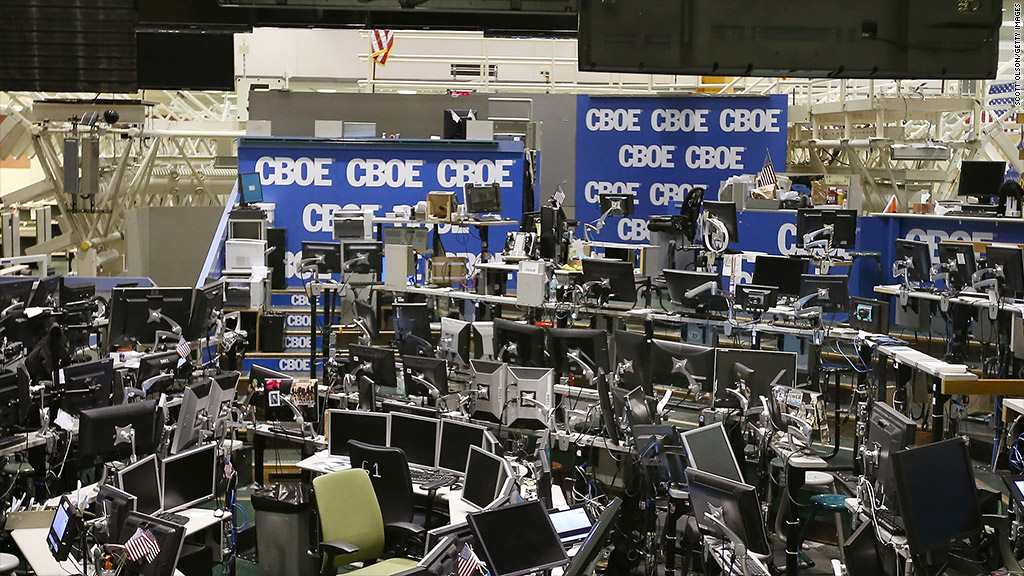
\includegraphics[width
		= 3cm]{ProgramsImages/130611131918-chicago-board-options-exchange-1024x576.jpg}}}
	
	\newcommand{\scoop}[1]{\parbox{#1}{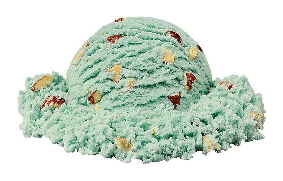
\includegraphics[width=#1]{IceCreamScoop.eps}}\xspace}
	\newcommand{\smallscoop}{\scoop{1cm}}
	\newcommand{\medscoop}{\scoop{1.8cm}}
	\newcommand{\largescoop}{\scoop{3cm}}
	\newcommand{\ICcone}[1]{\parbox{#1}{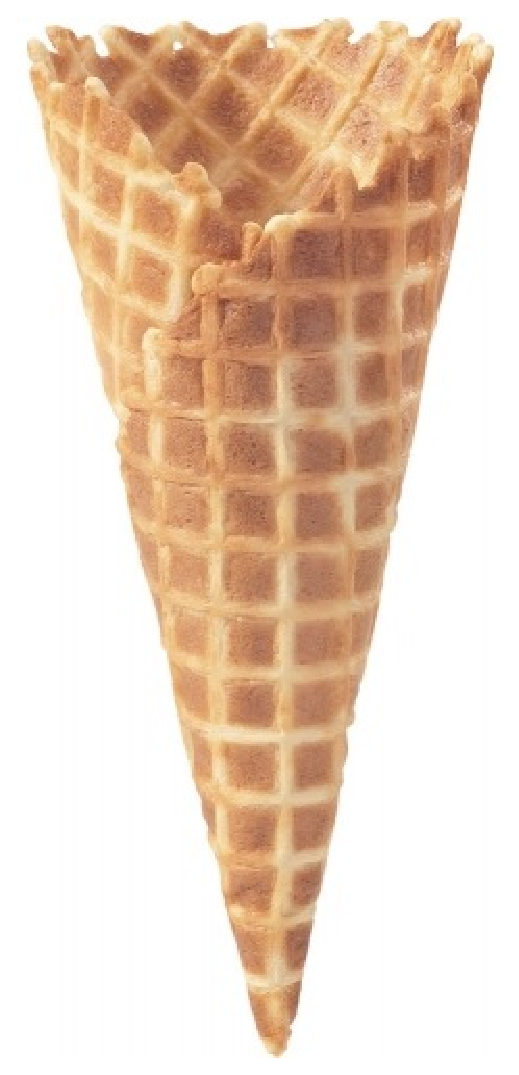
\includegraphics[width=#1,angle=270]{MediumWaffleCone.eps}}\xspace}
	\newcommand{\medcone}{\ICcone{1.2cm}}
	\newcommand{\largercone}{\parbox{2.2cm}{\vspace*{-0.2cm}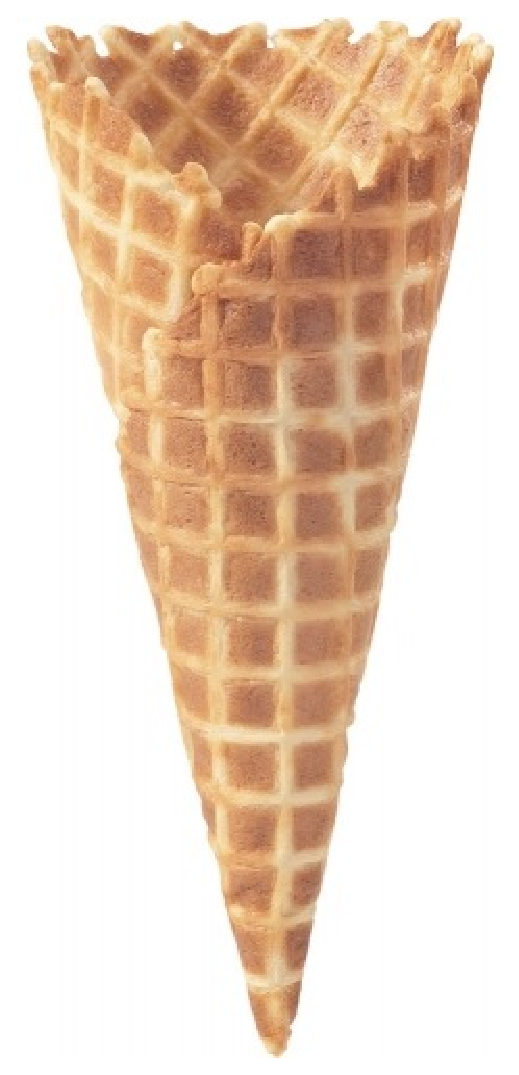
\includegraphics[width=1cm,angle=270]{MediumWaffleCone.eps}}\xspace}
	\newcommand{\largecone}{\ICcone{1.8cm}}
	\newcommand{\smallcone}{\parbox{0.65cm}{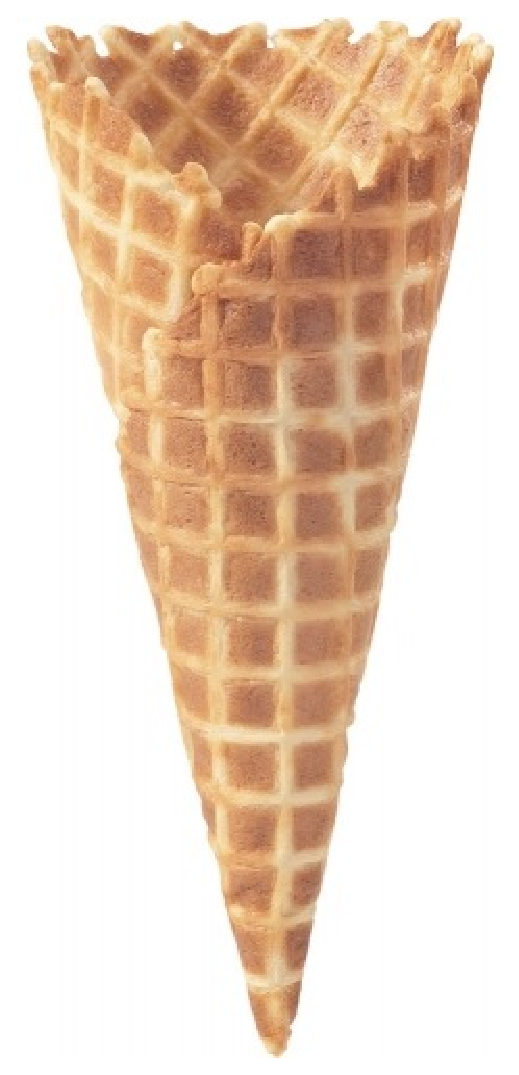
\includegraphics[width=0.3cm,angle=270]{MediumWaffleCone.eps}}\xspace}
	


\begin{document}
\everymath{\displaystyle}
\frame{\titlepage}

\finalthanksnote{
Thank you all for your participation \\
\uncover<2>{Thanks to Peter Kritzer and Annette Weihs for doing all the work of organizing}}


\thankyouframe

\section{Introduction}

\begin{frame}{Context}

\vspace{-3ex}

\centerline{
    \begin{tabular}{>{\vspace{-1.7ex}\raggedleft}p{0.2\textwidth}@{\qquad}p{0.33\textwidth}@{\qquad}p{0.27\textwidth}}
    & \alert{Tidbits from talks this week} & \alert{My reponse} \tabularnewline
    \toprule
    \alert{Henryk, Klaus, Greg, Stefan, Erich, \ldots} & Many results for $f \in \smallscoop$  &
    Let's obtain analogous results for $f \in \smallcone$? \tabularnewline[4ex]
    \alert{Houman} & Let's \alert{learn} the appropriate kernel from the function data & Will only work for nice functions in a \smallcone \tabularnewline[2ex]
    \alert{Klaus} & ``This adaptive algorithm has \alert{no theory}''  & We want to construct adaptive algorithms \alert{with theory} \tabularnewline[2ex]
    \alert{Henryk} & Tractability & Yes! \tabularnewline[2ex]
    \alert{Greg} & POD weights & Yes! \tabularnewline[2ex]
    \alert{Mac} & Function values are expensive & Yes!
    \end{tabular}}
\end{frame}



\begin{frame}{Multivariate Linear Problems}
\vspace{-3ex}
\begin{tabular}{p{0.47\textwidth}p{0.5\textwidth}}
Given $f \in \cf$ find $S(f) \in \cg$, where \\
$\sol: \cf \to \cg$ is linear, e.g., 
\begin{gather*}
    S(f) = \int_{\reals^d} f(\vx) \, \varrho(\vx) \, \dif \vx\\
    S(f) = f\\
    S(f) = \frac{\partial f}{\partial x_1} \\
    - \nabla^2 S(f) = f, \ \  S(f) = 0 \text{ on boundary}
\end{gather*}
&
\vspace{-7ex}
\alert{Successful algorithms}
\vspace{-3ex}
\begin{multline*}
    \ca(\cc,\Lambda) : = \{\app: \cc \times (0,\infty) \to \cg \text{ such that } \\
\norm[\cg]{\sol(f) - \app(f,\varepsilon) } \le \varepsilon \ \ \forall f \in \cc \subseteq \cf, \ \varepsilon > 0 \}
\end{multline*}

\vspace{-1ex}
where $\app(f,\varepsilon)$ depends on \alert{function values}, $\LambdaStd$, \alert{Fourier coefficients}, $\LambdaSer$, or \alert{any linear functionals}, $\LambdaAll$, e.g., 

\vspace{-4ex}
\begin{gather*}
    \Sapp(f,n) = \sum_{i=1}^n f(\vx_i) \, g_i, \quad g_i \in \cg \\
    \Sapp(f,n) = \sum_{i=1}^n \hf_i \, g_i, \quad g_i \in \cg \\
    \Sapp(f,n) = \sum_{i=1}^n L_i(f) \, g_i, \quad g_i \in \cg \\
\end{gather*}

\vspace{-5ex}
\hfill \hfill \alert{$\app(f,\varepsilon) = \Sapp(f,n) + $ stopping criterion}\newline
\phantom{a} \hfill \hfill \alert{$\cc$ is a \smallcone}

\end{tabular}
    
\end{frame}

\begin{frame}{Issues}

\vspace{-3ex}

\begin{tabular}{p{0.47\textwidth}p{0.5\textwidth}}
Given $f \in \cf$ find $S(f) \in \cg$, where \\
$\sol: \cf \to \cg$ is linear

\bigskip

\alert{Successful algorithms}
\vspace{-2ex}
\begin{multline*}
    \ca(\cc,\Lambda) : = \{\app: \cc \times (0,\infty) \to \cg \text{ such that } \\
\norm[\cg]{\sol(f) - \app(f,\varepsilon) } \le \varepsilon \ \ \forall f \in \cc \subseteq \cf, \ \varepsilon > 0 \}
\end{multline*}

\vspace{-1ex}
where $\app(f,\varepsilon)$ depends on \alert{function values}, $\LambdaStd$, \alert{Fourier coefficients}, $\LambdaSer$, or \alert{any linear functionals}, $\LambdaAll$
&

\vspace{-9ex}
\uncover<1->{\alert{Solvability}\footfullcite{KunEtal19a}: $\ca(\cc,\Lambda) \ne \emptyset$

\smallskip

\alert{Construction}: Find $\app \in \ca(\cc,\Lambda)$}

\smallskip

\uncover<2->{\alert{Cost}: $\cost(\app,f,\varepsilon) = $ \# of function data
\newline
 $\cost(\app,\cc,\varepsilon, \rho) = \max_{f \in \cc \cap \cb_{\rho}} \cost(\app,f,\varepsilon)$
 \newline
 $\cb_{\rho} := \{f \in \cf : \norm[\cf]{f} \le \rho \}$
 
 \smallskip

\alert{Complexity}\footfullcite{TraWasWoz88}: $\comp(\ca(\cc,\Lambda),\varepsilon,\rho)$ 
\newline \phantom{a} \hfill \hfill $= \min_{\app \in \ca(\cc,\Lambda)} \cost(\app,\cc,\varepsilon, \rho)$

\alert{Optimality}:  \newline \phantom{a} \hfill \hfill $\cost(\app,\cc,\varepsilon, \rho) \le \comp(\ca(\cc,\Lambda),\alert{\omega} \varepsilon,\rho)$}

\smallskip

\uncover<3->{\alert{Tractability}\footfullcite{NovWoz08a}: $\comp(\ca(\cc,\Lambda),\varepsilon, \rho) \le C \rho^p\varepsilon^{-p} d^{q} $}

\smallskip
\uncover<4->{\alert{Implementation} in open source software}

\vspace{-6ex}

\phantom{a}

\end{tabular}
    
\end{frame}

\begin{frame}[label = ConeFrame]{Cones}
\vspace{-4ex}
\begin{tabular}{>{\centering}m{0.4\textwidth}@{\qquad}>{\centering}m{0.4\textwidth}}
     \largescoop \hspace{-3cm}\raisebox{-4ex}{\color{red}\fontsize{100}{120}\selectfont $\times$} & 
      \largecone \tabularnewline
      Ball $\cb_{\rho} := \{f \in \cf : \norm[\cf]{f} \le \rho \}$ &
      \hspace{2cm} (Non-Convex) Cone $\cc$
\end{tabular}

\begin{itemize}
    \item Assume set of inputs, $\cc \subseteq \cf$, is a \alert{cone}, not a ball
    
    \item \alert{Cone} means $f \in \cc \implies af \in \cc \ \ \forall a \in \reals$
    
    \item \alert{Cones} are unbounded
    
    \item If we can bound the $\norm[\cg]{S(f) - \Sapp(f,n)}$ for $f \in $ \alert{cone}, then we can typically also bound the error  for $af$
    
    %\item Union of \alert{cones} is a \alert{cone}
    
    \item \alert{Philosophy:}  What we cannot observe about $f$ is not much worse than what we can observe about $f$
    
\end{itemize}

    
\end{frame}

\begin{frame}[label = BallsWontHelp]{``But I Like \smallscoop!''}

\vspace{-5ex}
How might you construct an\only<2>{\alert{adaptive}} algorithm if you insist on using \smallscoop?

\vspace{-2ex}
\begin{description}
    \item[Step 1] Pick with a default radius $\rho$, and \alert{assume} input $f \in \cb_{\rho}$
    
    \item[Step 2] Choose $n$ \alert{large enough} so that 
    
    \vspace{-4ex}
    \begin{multline*}
     \norm[\cg]{S(f) - \Sapp(f,n)} \le \norm[\cf\to \cg]{S - \Sapp(\cdot,n)} \rho \le \varepsilon \\
         \text{where } \Sapp(f,n) = \sum_{i=1}^n L_i(f) g_i
    \end{multline*}
    
    \vspace{-2ex}
    
    \item<2>[Step 3] Let $f_{\textup{min}} \in \cf$ be the \alert{minimum} norm interpolant of the data $L_1(f), \ldots, L_n(f)$
    
    \item[Step 4]  \uncover<2>{If $C\bignorm[\cf]{f_{\textup{min}}} \le \rho$ for some preset \alert{inflation} factor, $C$, \\}then return $A(f,\varepsilon) = \Sapp(f,n)$\uncover<2>{; \\otherwise, choose $\rho = 2C\bignorm[\cf]{f_{\textup{min}}}$, and go to Step 2}
\end{description}

\vspace{-2ex}

\uncover<2>{This succeeds for the \alert{cone} \smallcone defined as those functions in $\cf$ whose norms are not much larger than their minimum norm interpolants.}
    
\end{frame}


%\section{Solvability}
\begin{frame}{When Is $(S:\cc \subseteq \cf\to\cg,\Lambda)$ \emph{Solvable}?}

\vspace{-7ex}
\begin{multline*}
     \ca(\cc,\Lambda) : = \{\app: \cc \times (0,\infty) \to \cg \text{ such that } 
\norm[\cg]{\sol(f) - \app(f,\varepsilon) } \le \varepsilon \ \forall f \in \cc \subseteq \cf, \ \varepsilon > 0 \}
  \\
  \text{where $A(f,\varepsilon)$ depends on } \{L_i(f)\}_{i=1}^n \in \Lambda^n \subseteq \cf^{*n}
\end{multline*}

\vspace{-3ex}

\alert{Definition} \quad $(S:\cc \subseteq \cf\to\cg,\Lambda)$ \alert{solvable} $\iff \ca(\cc,\Lambda) \ne \emptyset$\\[1ex]
\alert{Lemma}  \quad $f_1, f_2 \in \cc$  and $A(f_1, \varepsilon) = A(f_2,\varepsilon) \implies \norm[\cg]{S(f_1-f_2)} \le 2\varepsilon$\\[1ex]
\alert{Corollary} \label{ZeroCorollary} \quad $(S:\cc \subseteq \cf\to\cg,\Lambda)$ \alert{solvable} and $\exists f \in \cc,\  \varepsilon > 0$ with $A(f,\varepsilon) = A(0,\varepsilon)$  \\ \hfill \hfill $\implies S(f) = 0$\\[1ex]
\alert{Theorem} \label{VectorSpaceThm}\quad $(S:\cc \subseteq \cf\to\cg,\Lambda)$ \alert{solvable} and $\cc$ is a \alert{vector space} \\ \hfill \hfill 
$\iff \exists \ n \in \naturals, \ \vL \in \Lambda^n, \ \vg \in \cg^n$ such that $S(f) = \sum_{i=1}^n L_i(f) g_i \ \forall f \in \cc$ \alert{exactly}   \hyperlink{VectorSpaceThmProof}{\beamergotobutton{Proof}}\\[1ex]
E.g. $\left(\int_{[0,1]^d} \cdot (\vx) \, \dif \vx: C^{1,\ldots,1}[0,1]^d\to\reals,\Lambda^{\textup{std/\alert{all}}}\right)$ is unsolvable/\alert{solvable}
    
\end{frame}

%\section{Series Spaces}

\begin{frame}{Inputs and Outputs}

\vspace{-8ex}
\begin{gather*}
    \text{\alert{Input: }} f = \sum_{\vj \in \cn} \hf(\vj) u_{\vj} , \qquad 
    \text{\alert{Output: }} g = \sum_{\vj \in \cn} \hg(\vj) v_{\vj}, \qquad S(u_{\vj}) = v_{\vj}, \\
    \text{E.g., Integration: } S(u_{\vj}) = \int_{[0,1]^d} u_\vj (\vx) \, \dif \vx  = v_\vj, \qquad  \text{Function recovery: } S(u_{\vj}) = u_{\vj} = v_{\vj}, \qquad\\
    \text{\alert{Fixed sample size algorithm: }} \Sapp(f,n) = \sum_{i=1}^n L_i(f) g_i   \\
    \alert{\app(f,\varepsilon) = \Sapp(f,n) + \text{ stopping criterion}}
\end{gather*}

\vspace{-1ex}

Three scenarios presented here:

\vspace{-3ex}
\begin{description}[\labelwidth = 2cm]
\item[Integration] use $\LambdaStd$, but cost, complexity, etc. lacking
\item[General Linear Problems] use $\LambdaSer$, have cost, complexity, and optimality
\item[Function Approximation] use $\LambdaSer$, learn coordinate and smoothness weights
\end{description}


\end{frame}


\section{Integration}


\begin{frame}{Integration Using Function Values, $\LambdaStd$\footfullcite{DicEtal14a}}

\vspace{-7ex}

\begin{align*}
    S(f) & = \int_{[0,1]^d} f(\vx) \, \dif \vx\\[2ex]
    f &= \sum_{\vj \in \cn} \hf(\vj) u_{\vj}, \qquad
    u_{\vj} = \text{Cosine/Sine or Walsh}, \qquad S(u_{\vj}) = \delta_{\vj,\vzero}\\
    &\begin{array}{l}\Sapp(f,n) = \frac 1n \sum_{i=1}^n f(\vx_i)  \\[4ex]
    \abs{S(f) - \Sapp(f,n)} \le \sum_{\vzero \ne \vj \in \text{dual set}} \bigabs{\hf(\vj)}
    \end{array}
    \quad \raisebox{-8ex}{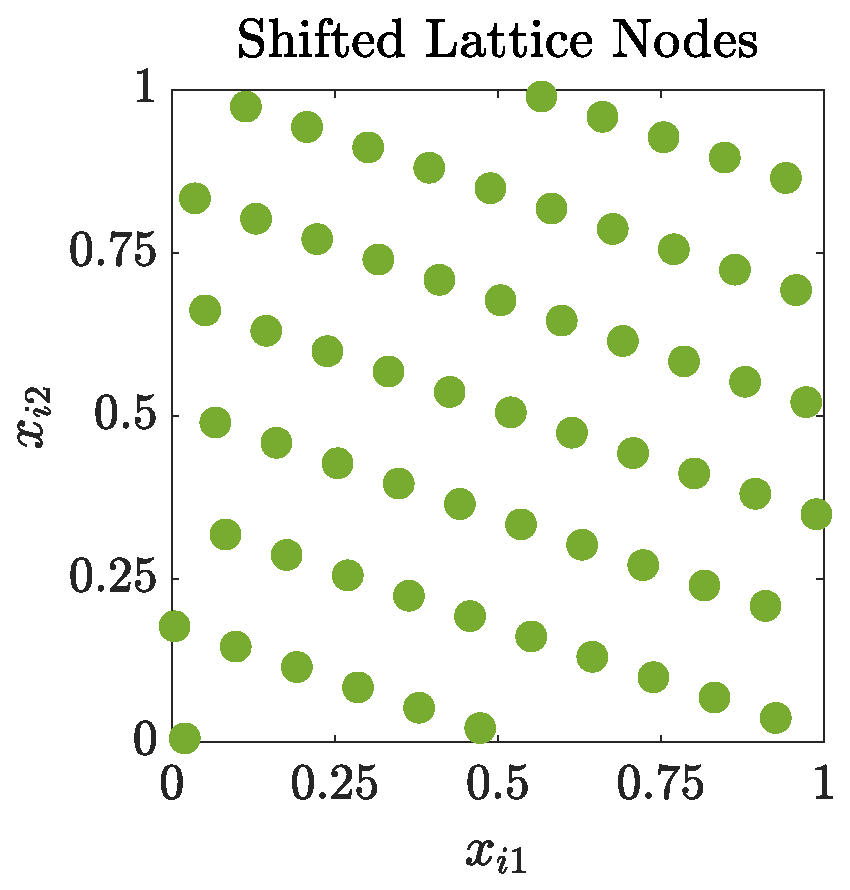
\includegraphics[width=3cm]{ProgramsImages/ShiftedLatticePoints.eps} \qquad
    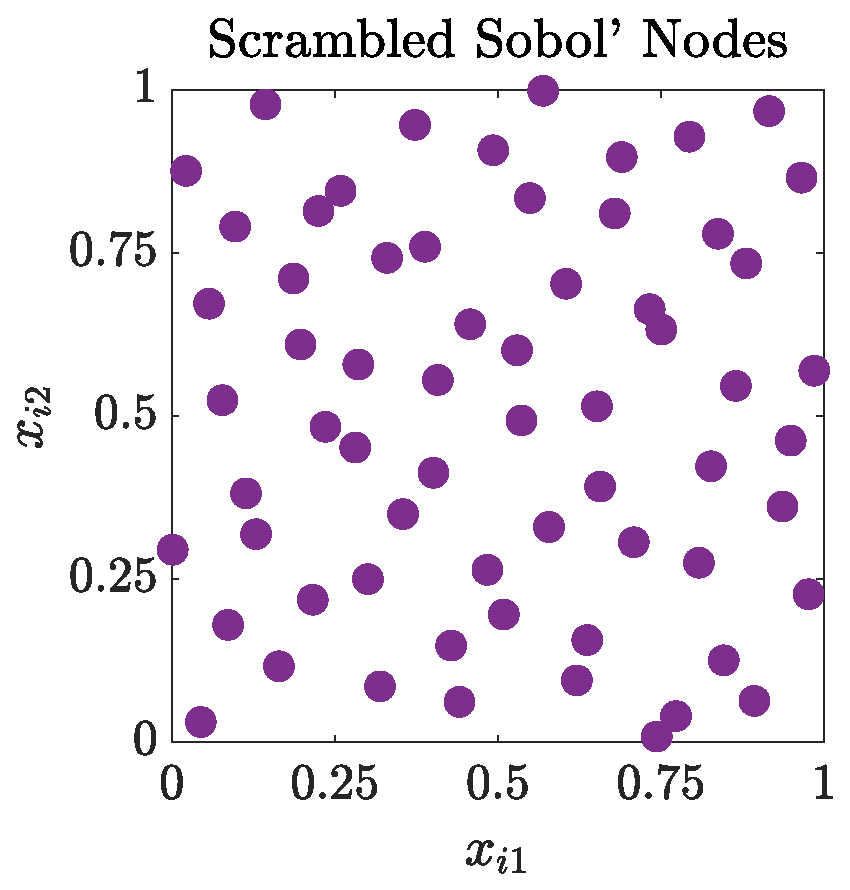
\includegraphics[width=3cm]{ProgramsImages/SSobolPoints.eps}}
\end{align*}

\end{frame}

\begin{frame}{Complex Exponential and Walsh Bases for Cubature}
\vspace{-3ex}
	\begin{tabular}{>{\centering}m{0.18\textwidth}>{\centering}m{0.18\textwidth}>{\centering}m{0.18\textwidth}>{\centering}m{0.18\textwidth}>{\centering}m{0.18\textwidth}}
		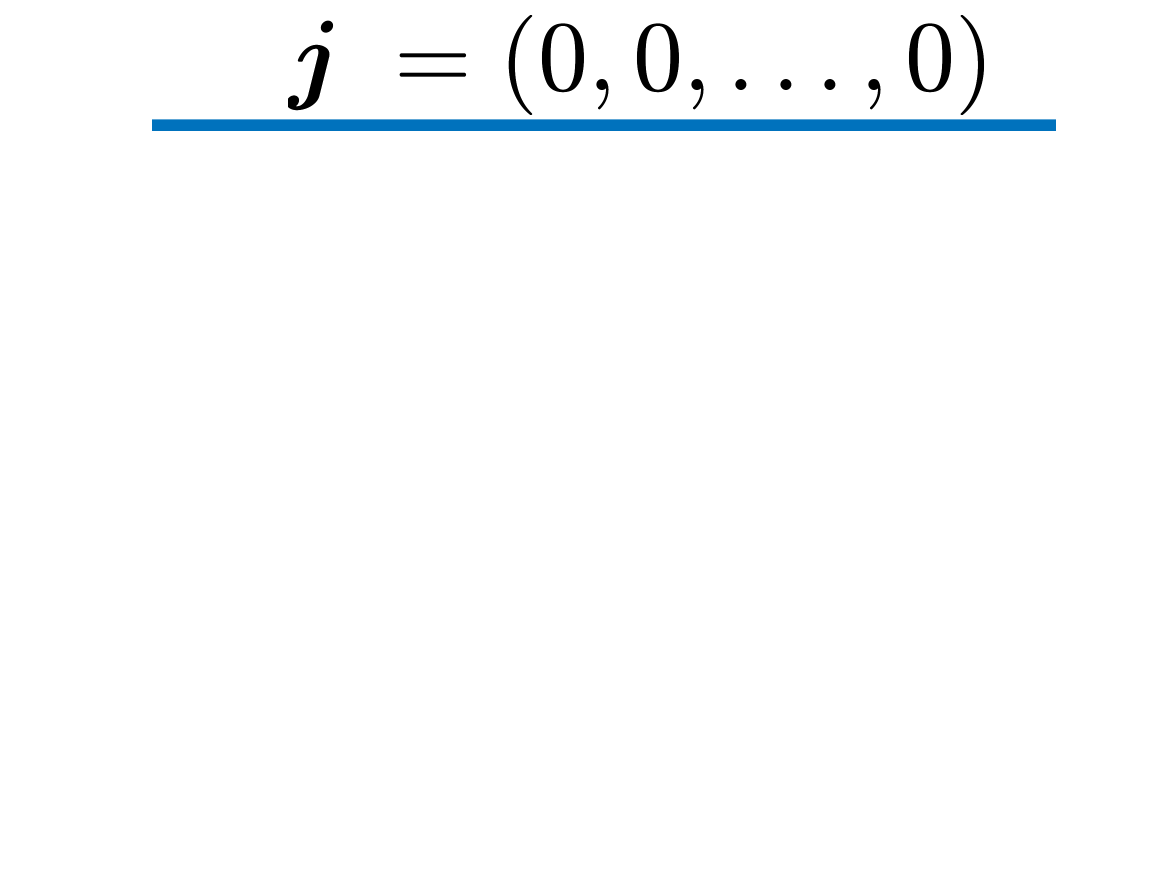
\includegraphics[width =0.18\textwidth]{ProgramsImages/CosineSine_Degree_0.png}  &
		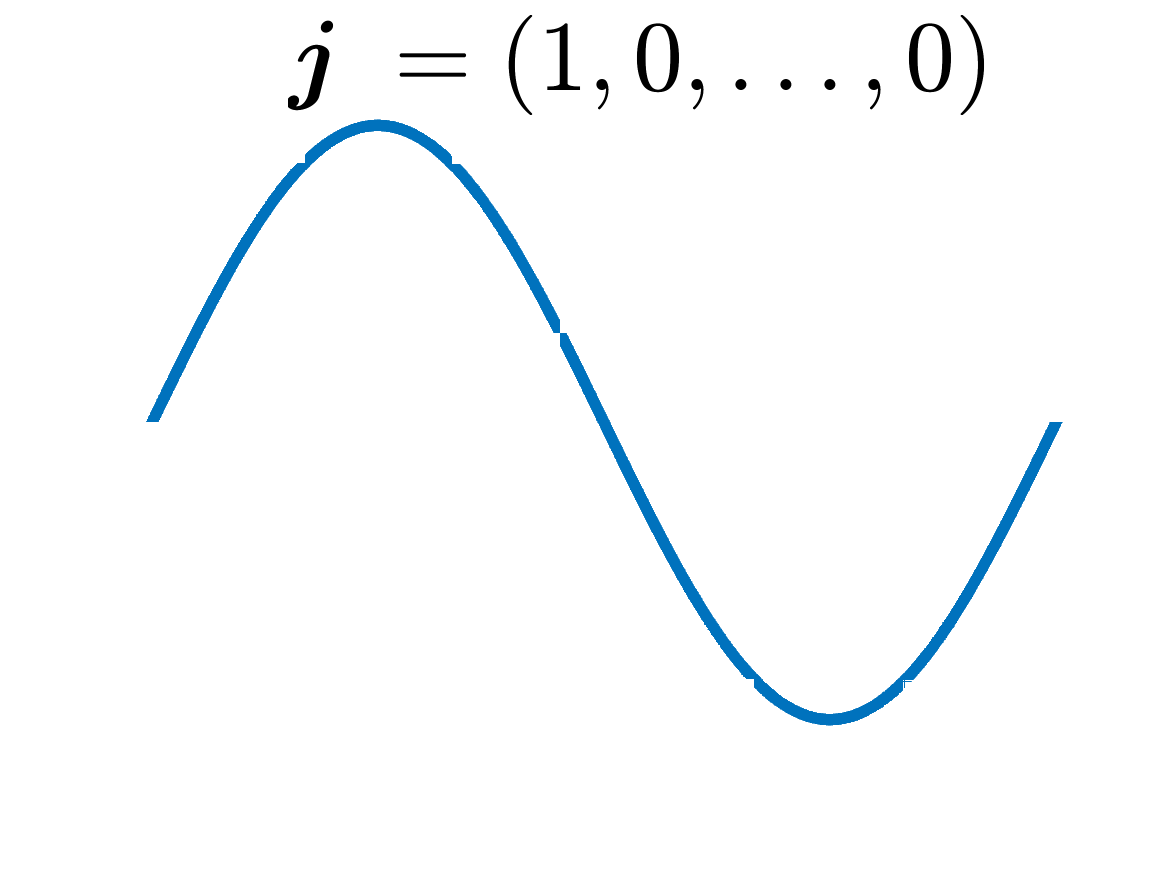
\includegraphics[width =0.18\textwidth]{ProgramsImages/CosineSine_Degree_1.png}  &
		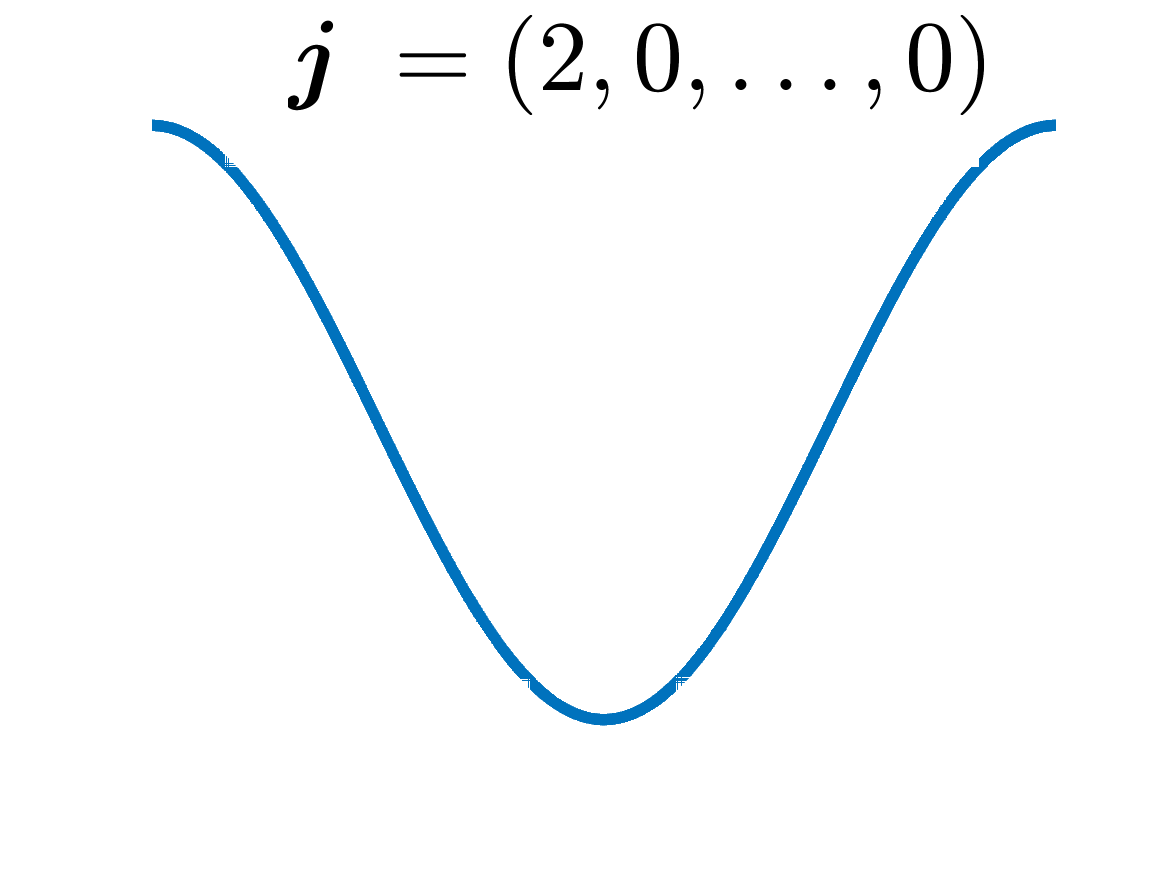
\includegraphics[width =0.18\textwidth]{ProgramsImages/CosineSine_Degree_2.png}  &
		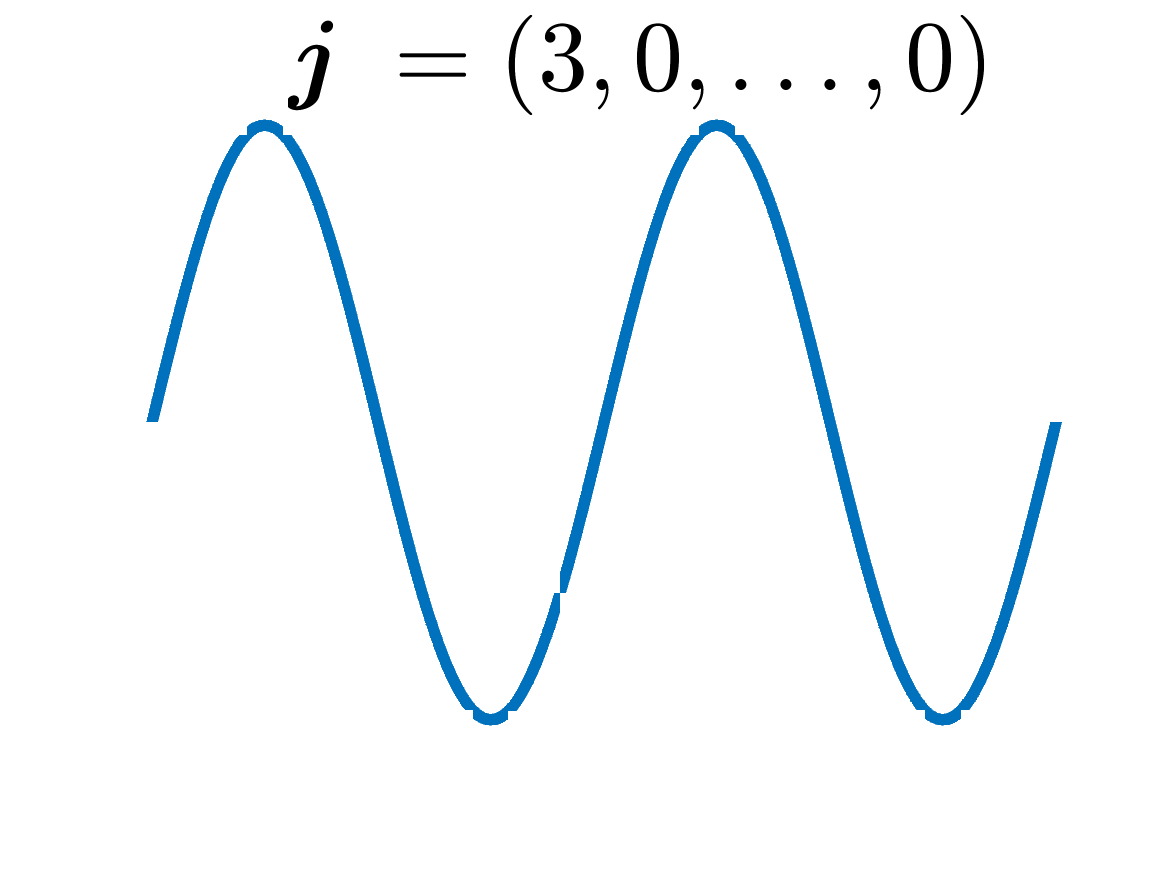
\includegraphics[width =0.18\textwidth]{ProgramsImages/CosineSine_Degree_3.png}  &
		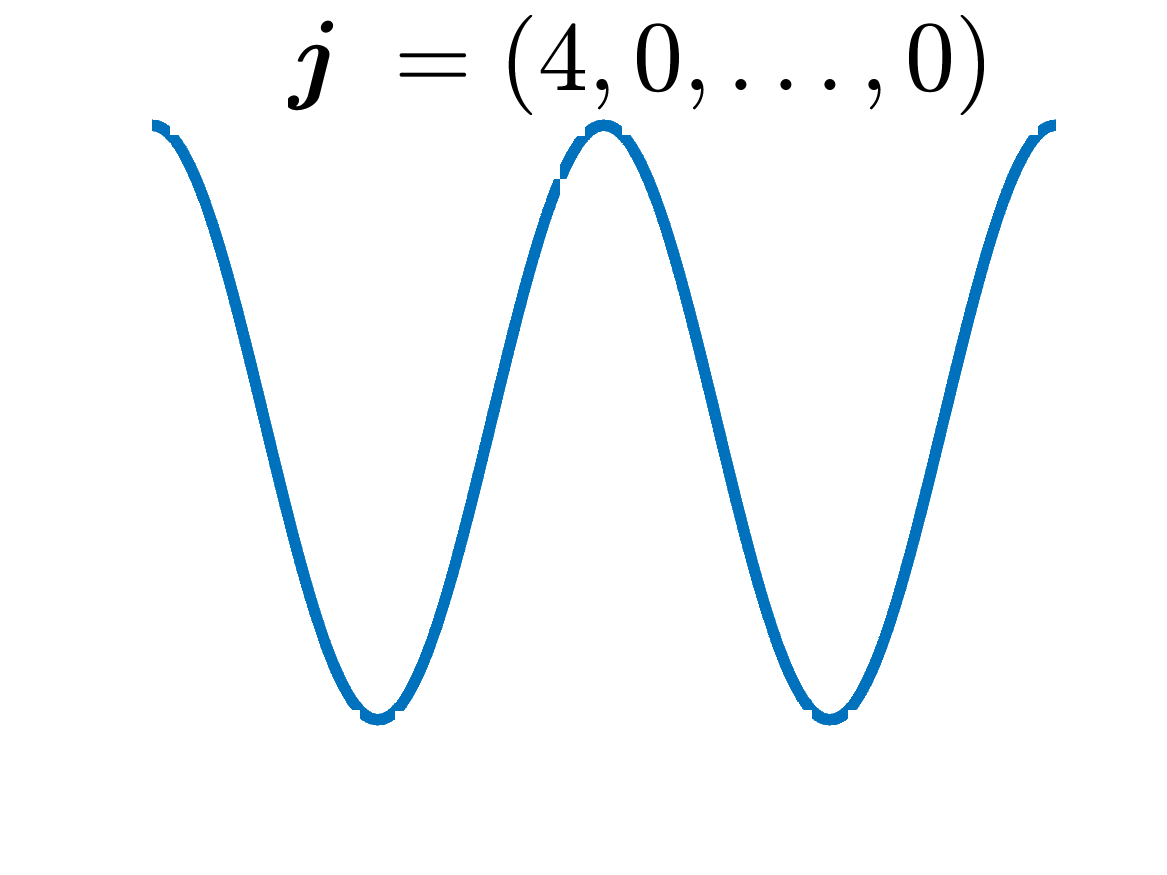
\includegraphics[width =0.18\textwidth]{ProgramsImages/CosineSine_Degree_4.png} 
	\tabularnewline[-7ex]
	Cosine \& Sine
	\tabularnewline
	\tabularnewline
		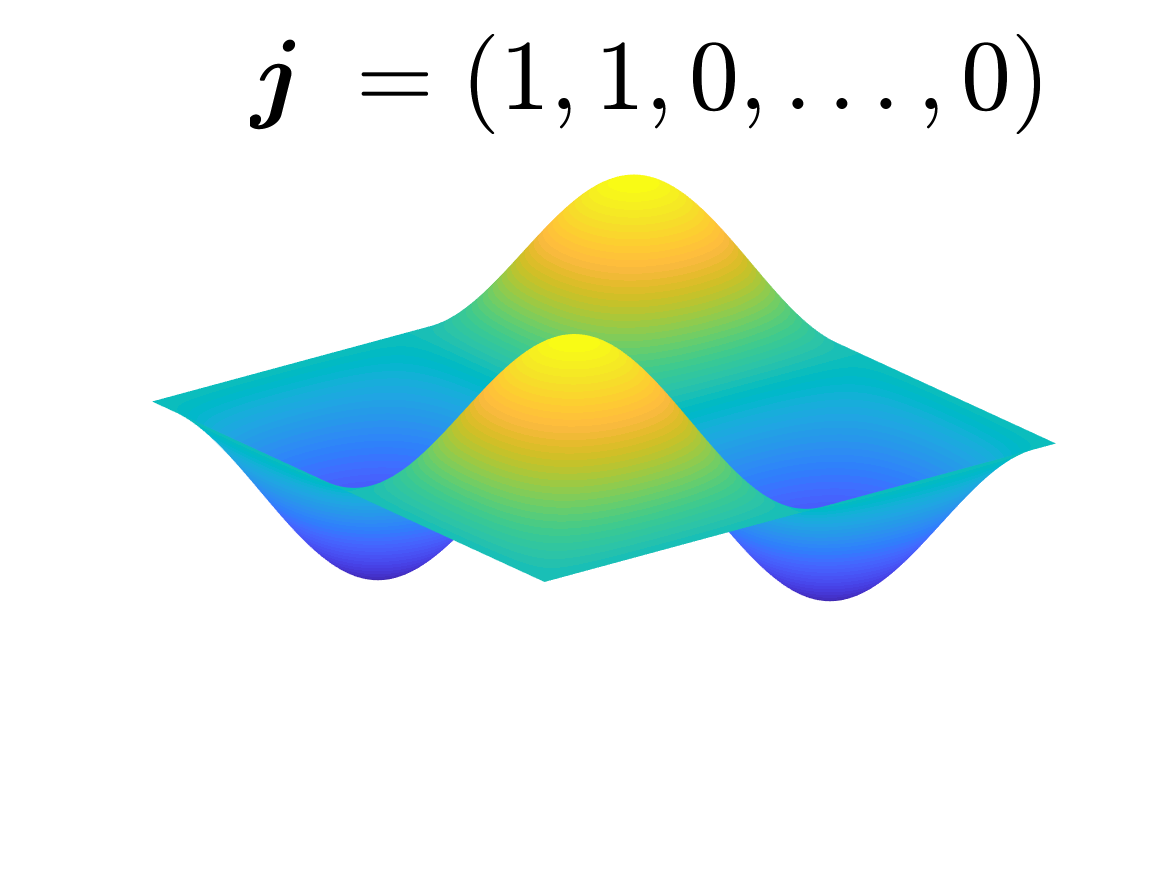
\includegraphics[width =0.18\textwidth]{ProgramsImages/CosineSine_Degree_1_1.png}  &
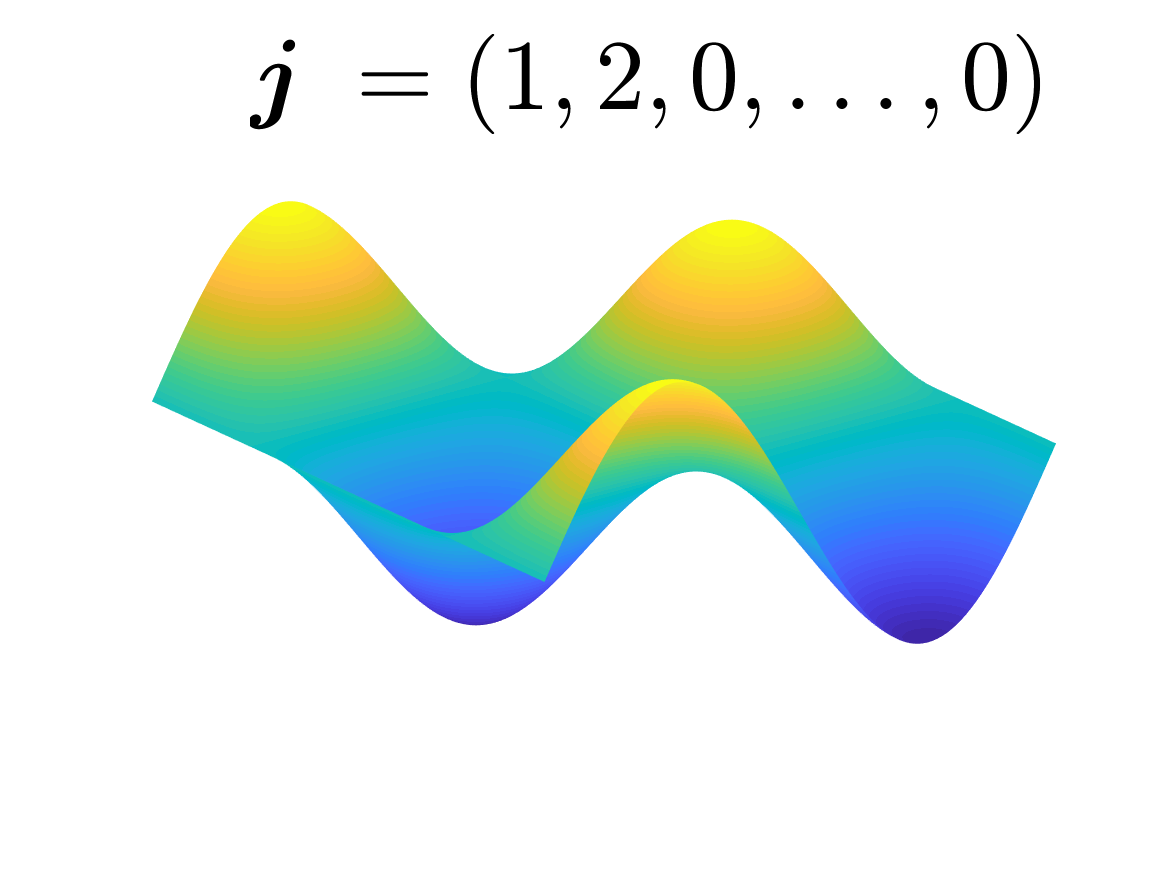
\includegraphics[width =0.18\textwidth]{ProgramsImages/CosineSine_Degree_1_2.png}  &
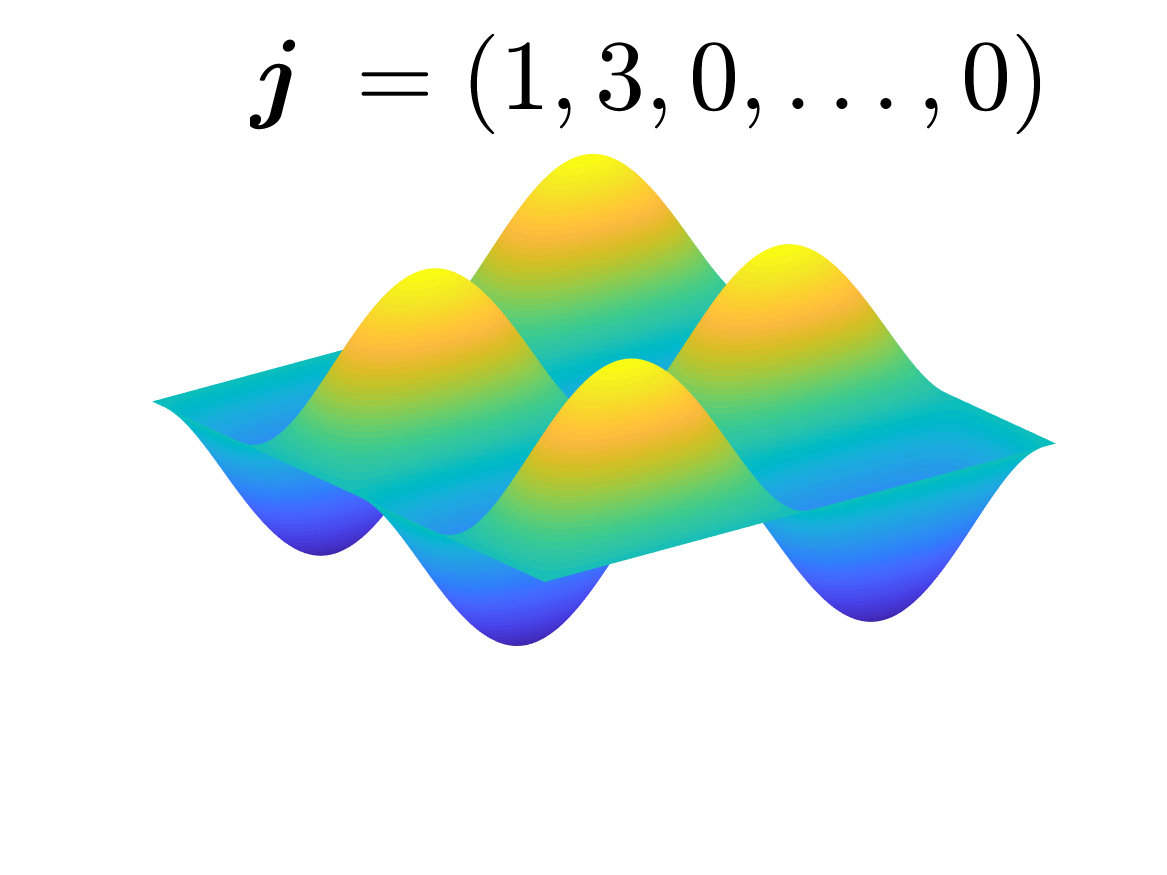
\includegraphics[width =0.18\textwidth]{ProgramsImages/CosineSine_Degree_1_3.png}  &
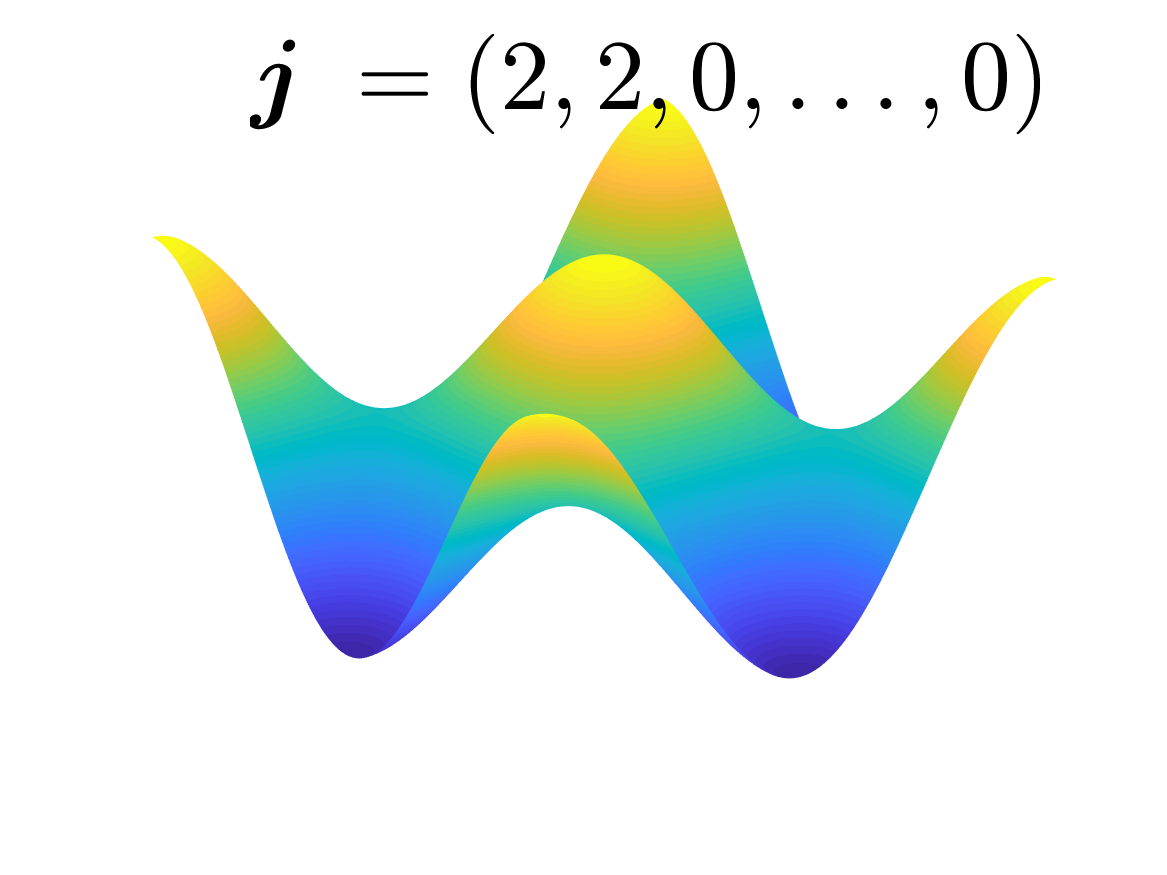
\includegraphics[width =0.18\textwidth]{ProgramsImages/CosineSine_Degree_2_2.png}  &
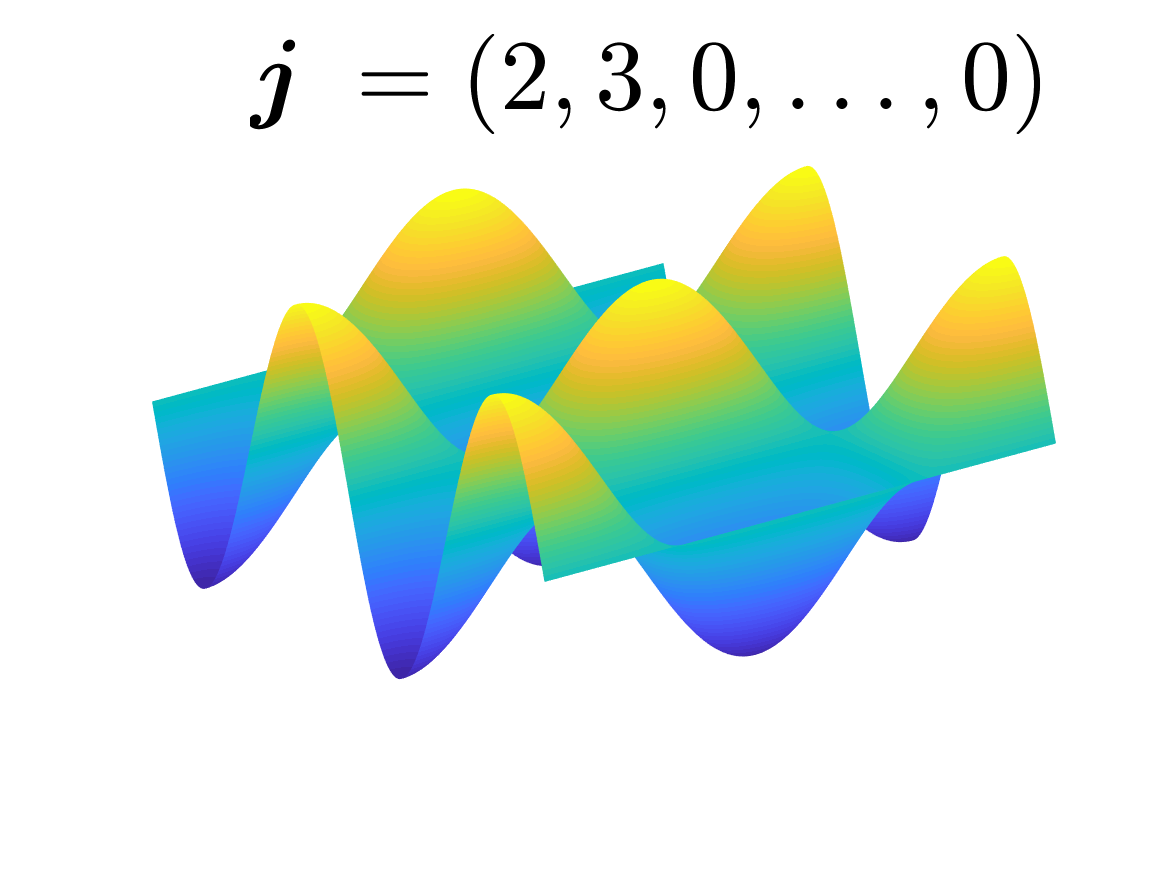
\includegraphics[width =0.18\textwidth]{ProgramsImages/CosineSine_Degree_2_3.png} 
\tabularnewline[0ex]
		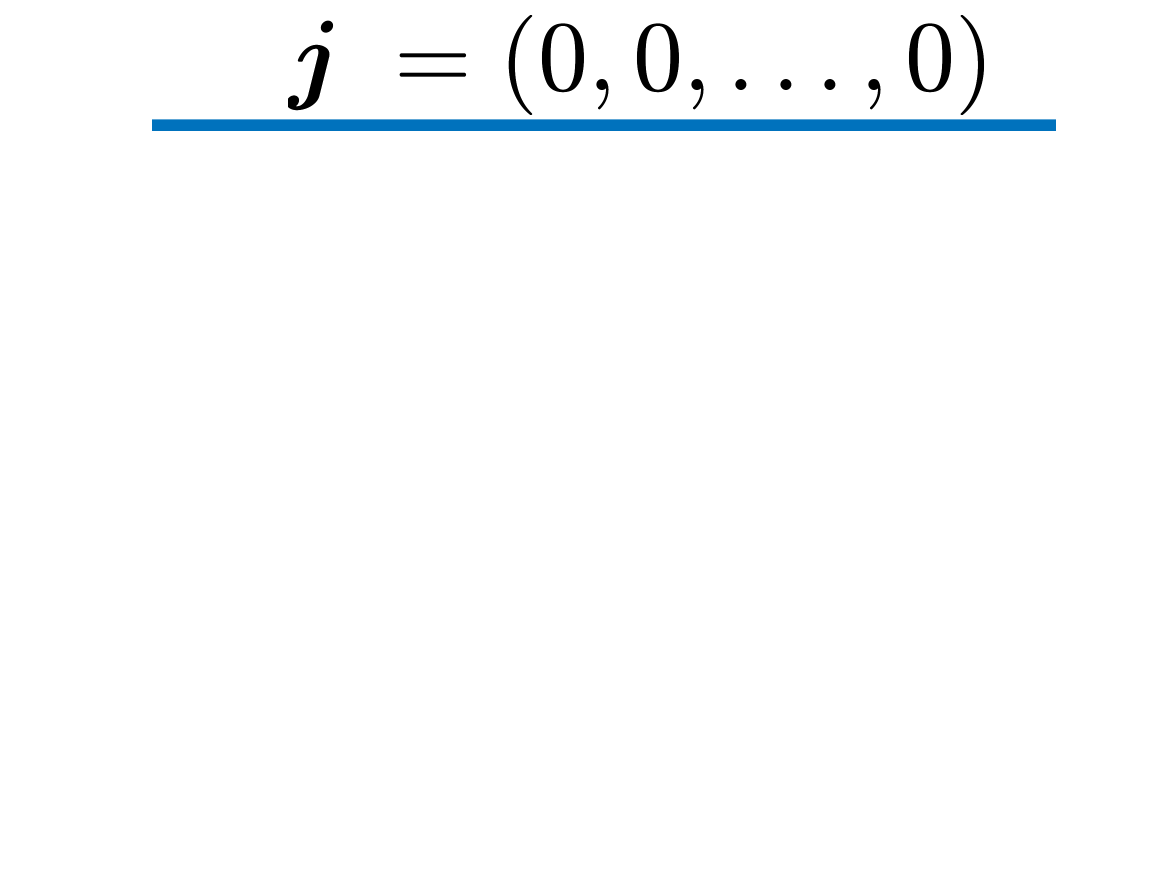
\includegraphics[width =0.18\textwidth]{ProgramsImages/Walsh_Degree_0.png}  &
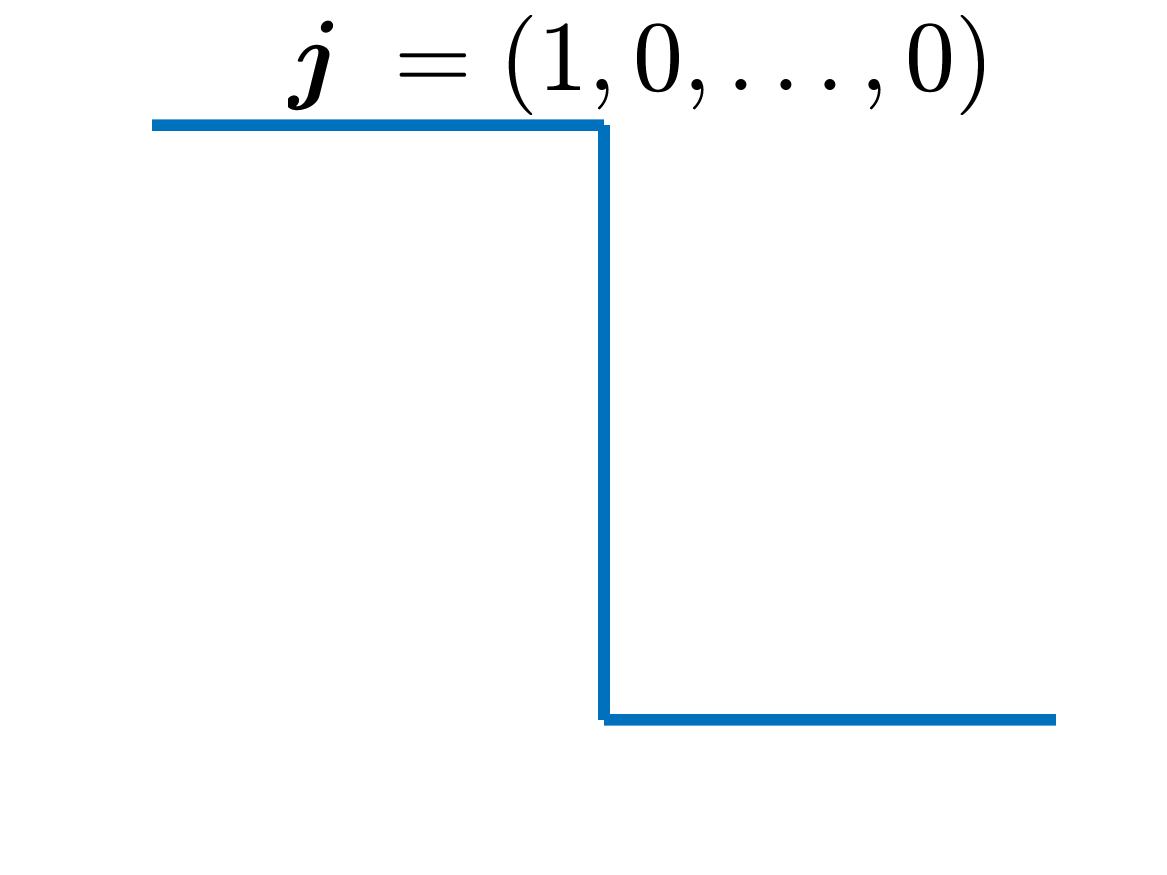
\includegraphics[width =0.18\textwidth]{ProgramsImages/Walsh_Degree_1.png}  &
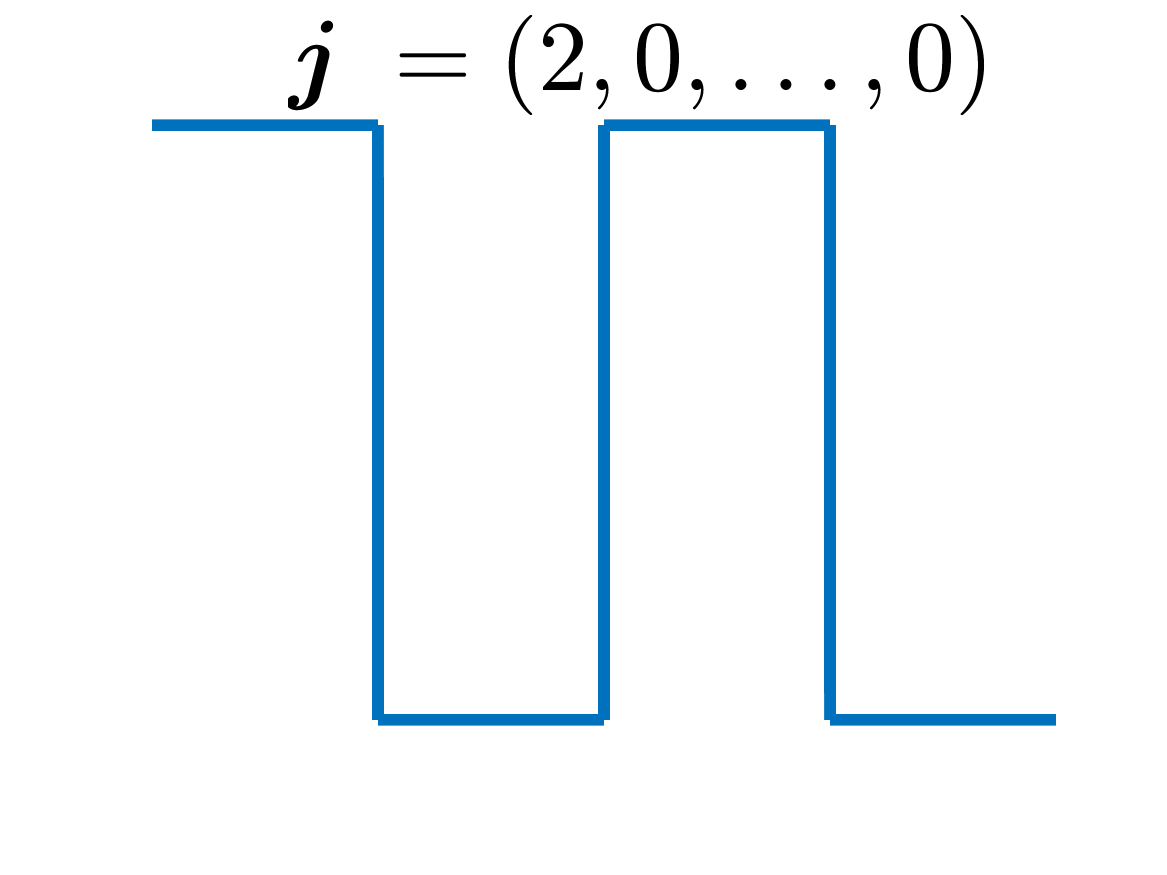
\includegraphics[width =0.18\textwidth]{ProgramsImages/Walsh_Degree_2.png}  &
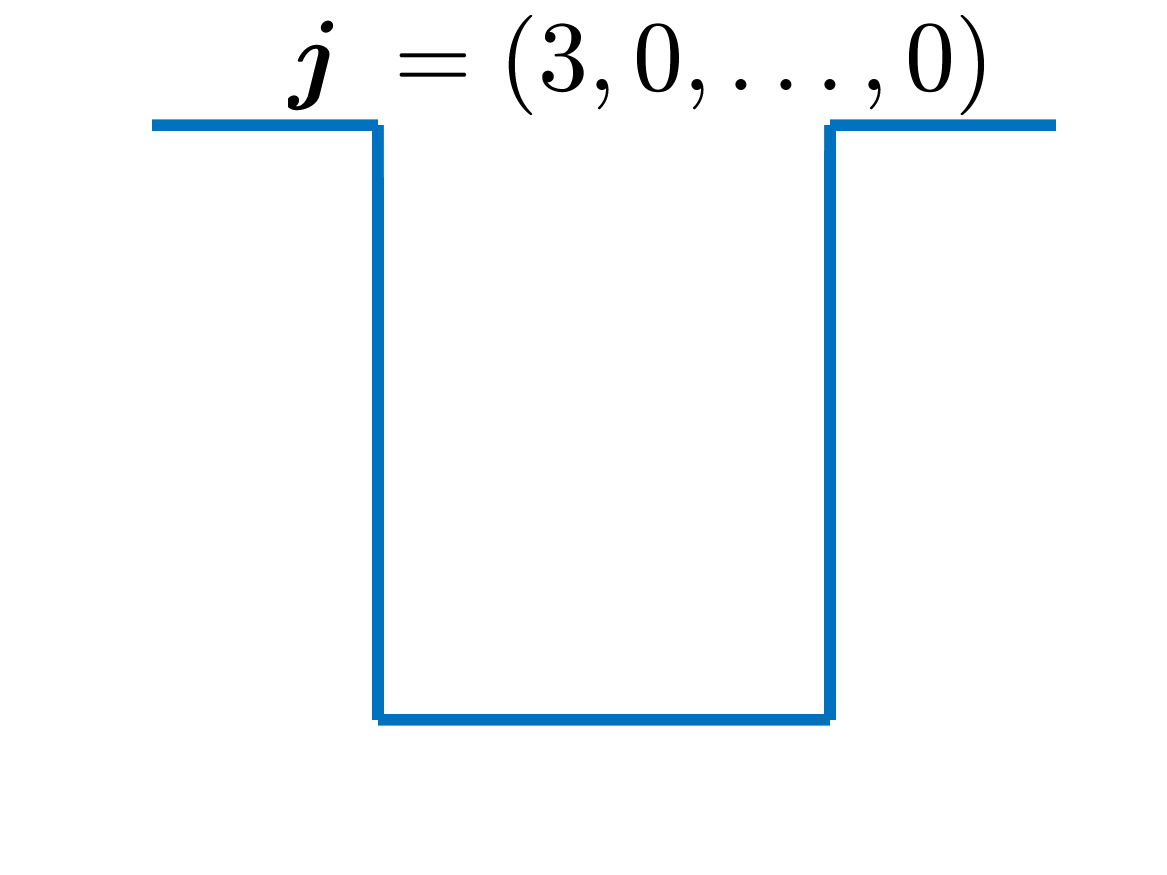
\includegraphics[width =0.18\textwidth]{ProgramsImages/Walsh_Degree_3.png}  &
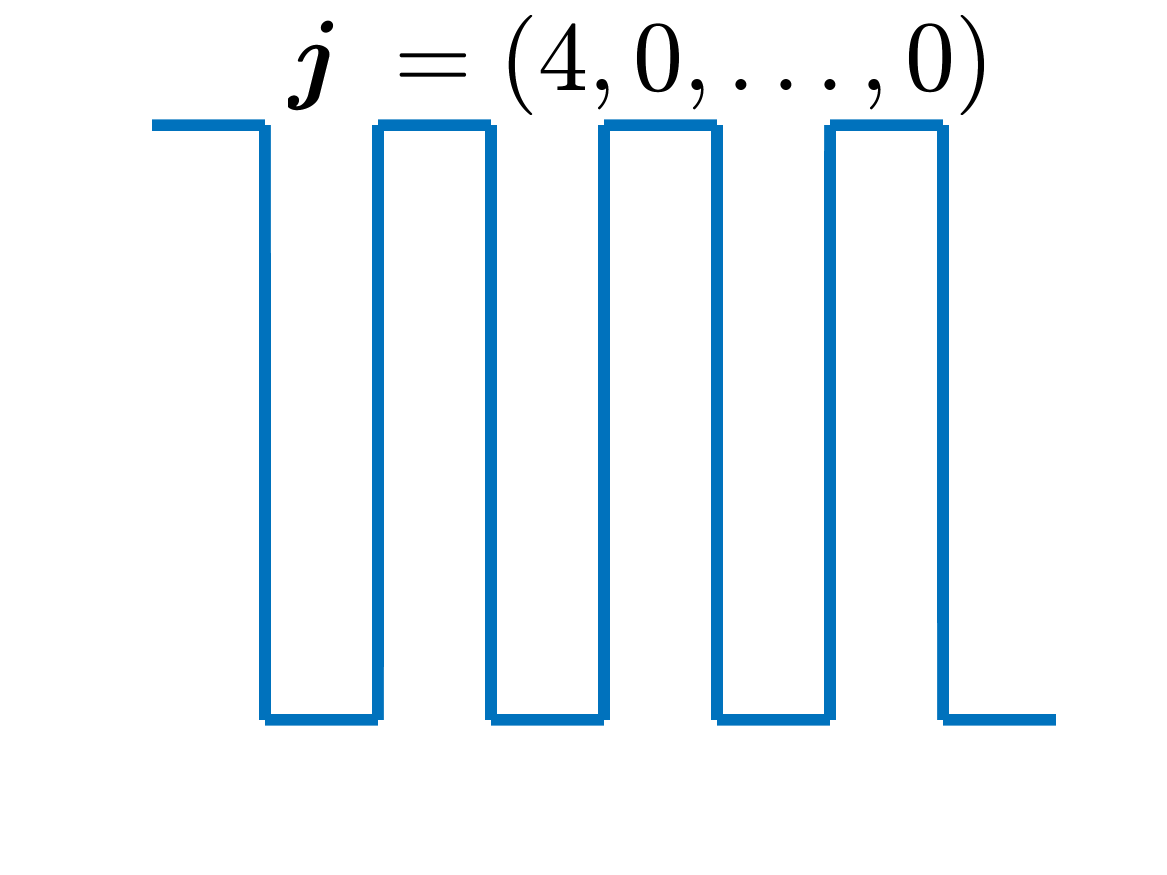
\includegraphics[width =0.18\textwidth]{ProgramsImages/Walsh_Degree_4.png} 
\tabularnewline[-7ex]
Walsh \tabularnewline
\tabularnewline
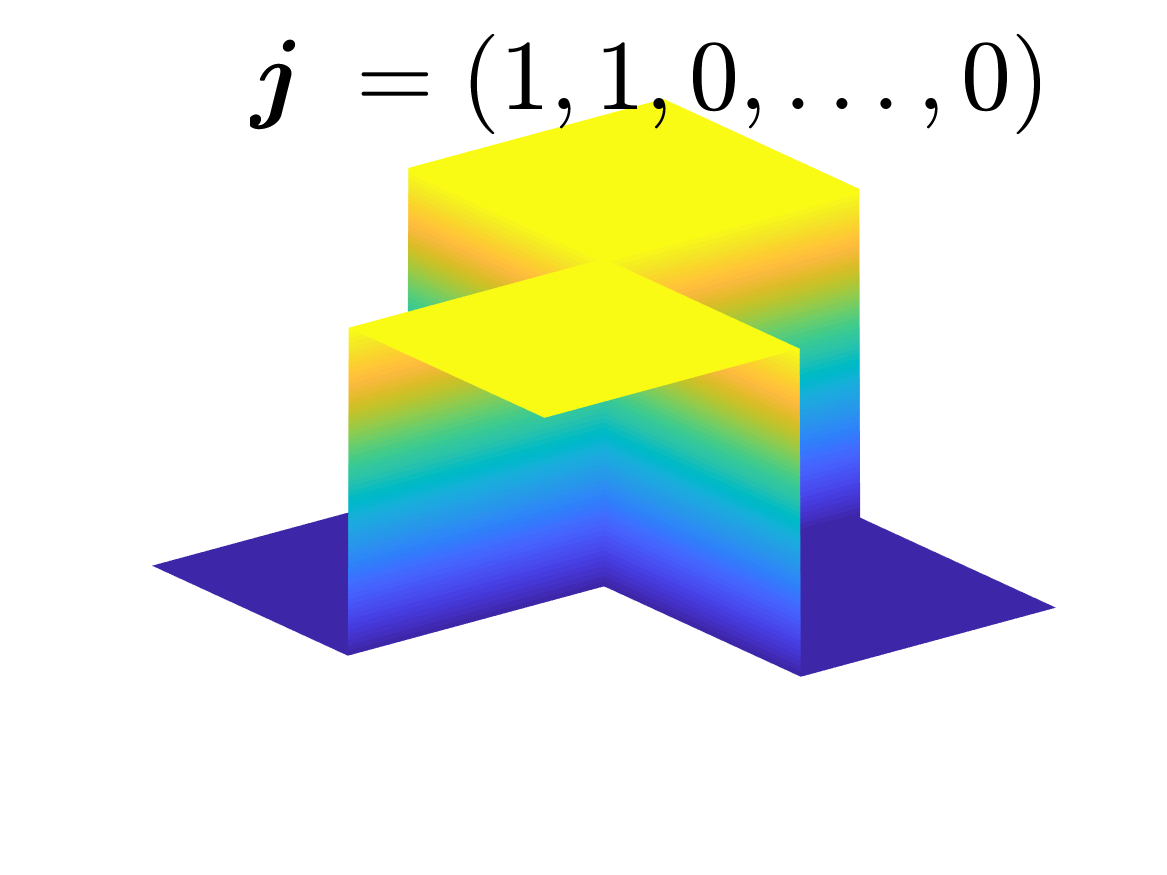
\includegraphics[width =0.18\textwidth]{ProgramsImages/Walsh_Degree_1_1.png}  &
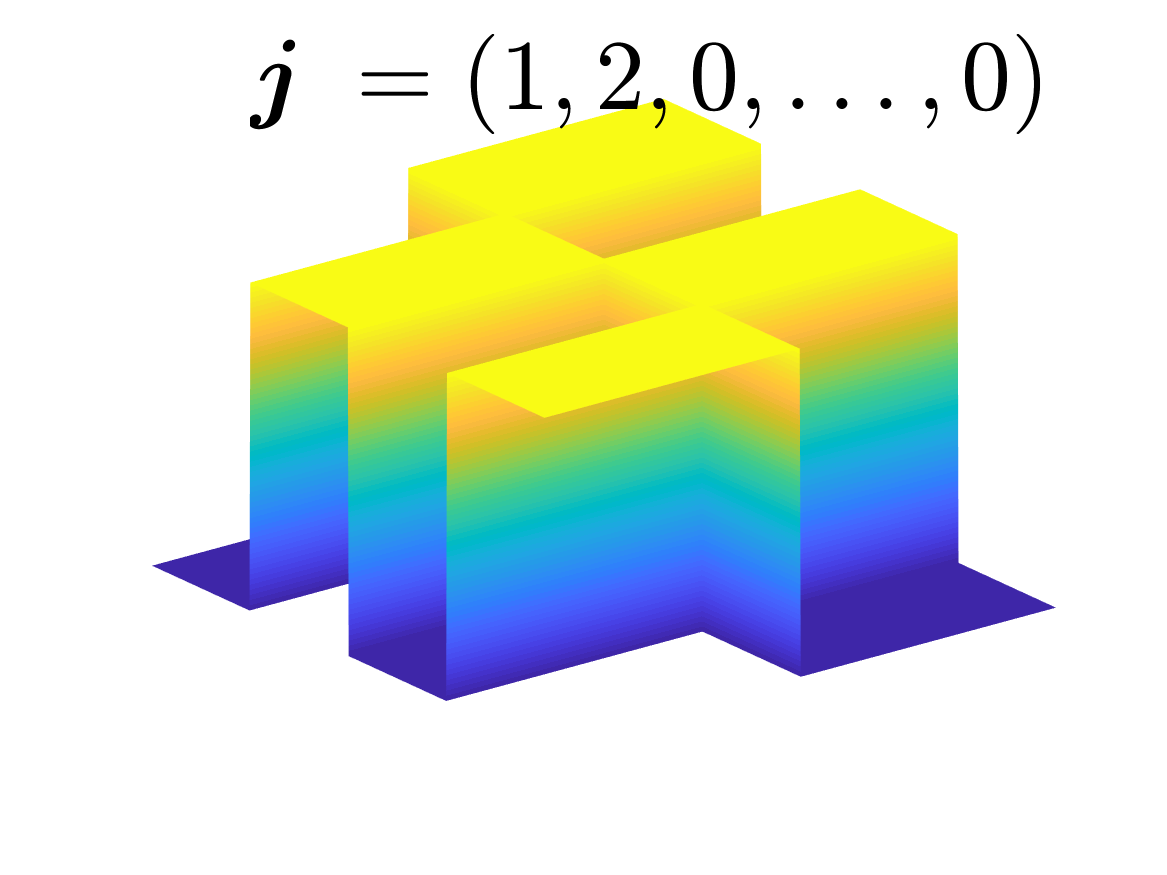
\includegraphics[width =0.18\textwidth]{ProgramsImages/Walsh_Degree_1_2.png}  &
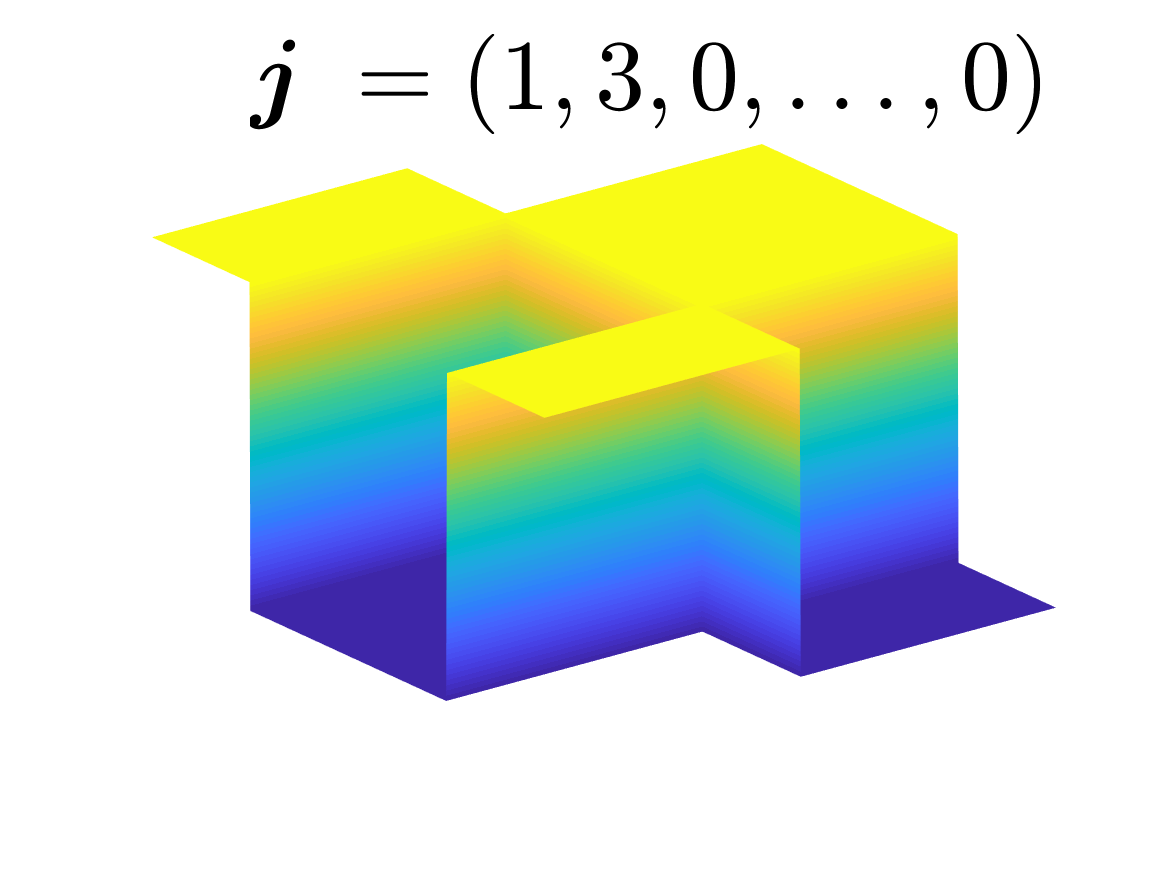
\includegraphics[width =0.18\textwidth]{ProgramsImages/Walsh_Degree_1_3.png}  &
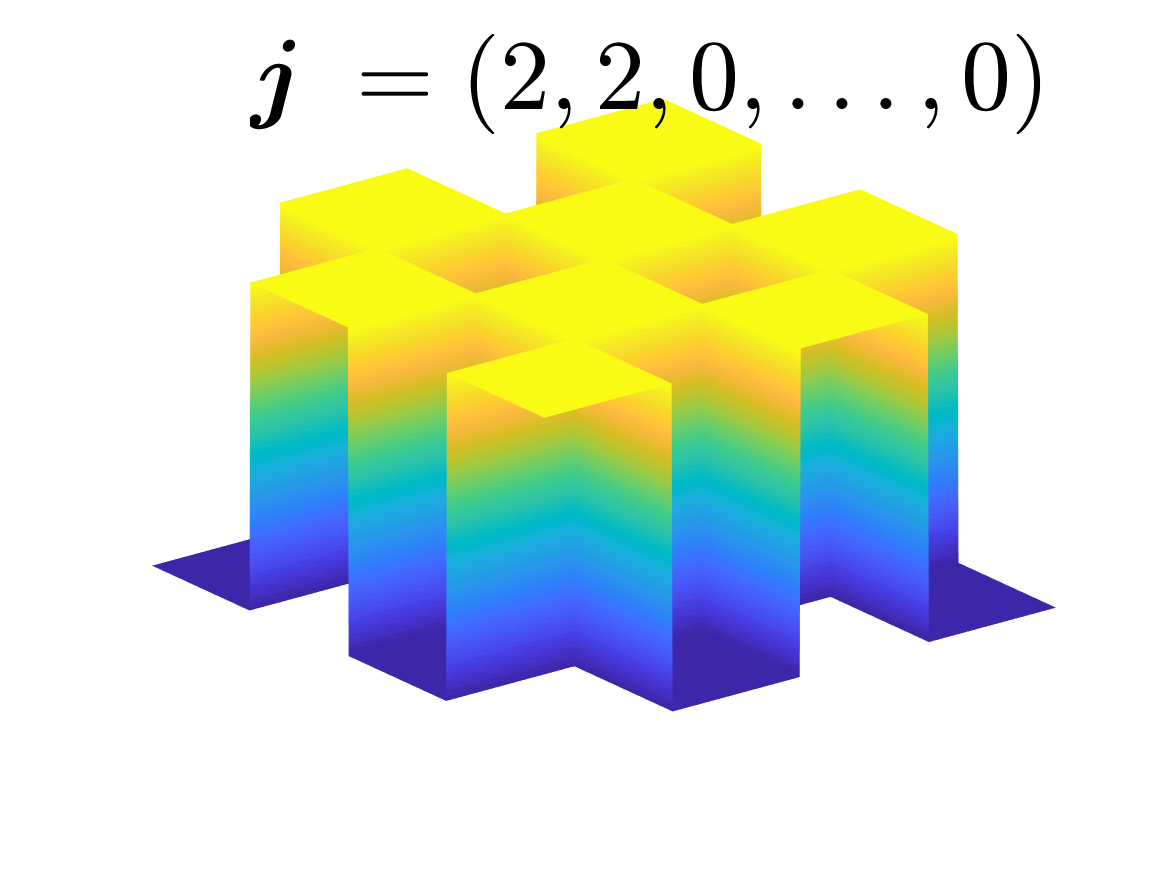
\includegraphics[width =0.18\textwidth]{ProgramsImages/Walsh_Degree_2_2.png}  &
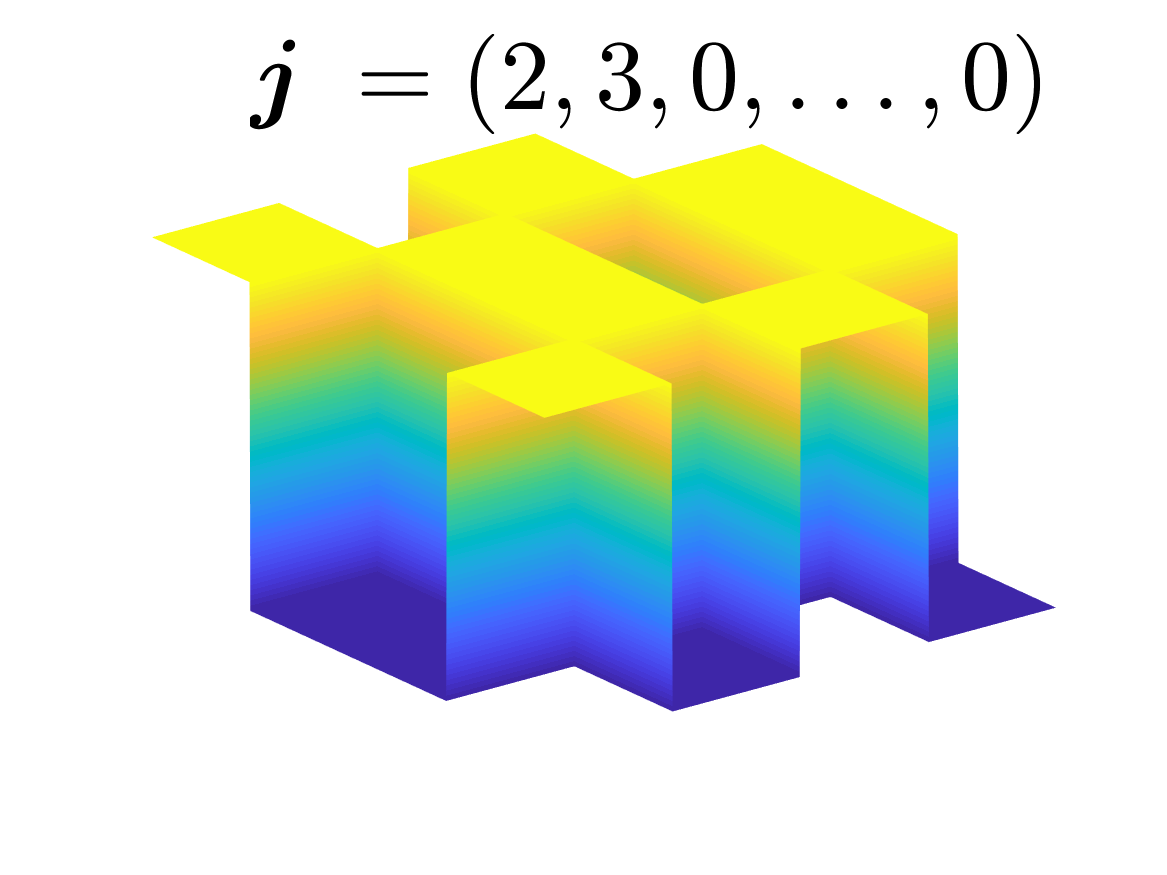
\includegraphics[width =0.18\textwidth]{ProgramsImages/Walsh_Degree_2_3.png} 
	\end{tabular}
\end{frame}



\begin{frame}{Cones of Integrands Whose Fourier Series Coefficients Decay Steadily\footfullcite{HicJim16a,JimHic16a}}

\vspace{-8ex}

\begin{align*}
n_0 & = 0, \quad n_k = 2^{k-1}, \ k \in \naturals, \qquad \vj \text{ ordered}, \quad \text{true coef.} = \hf(\vj) \approx \hf_{\text{disc}}(\vj) = \text{discrete coef.}\\
	 \sigma_k(f) & = \sum_{i=n_{k-1}+1}^{n_k}  \bigabs{\hf(\vj_i)}, \quad  \hsigma_{k,\ell}(f)  = \sum_{i=n_{k-1}+1}^{n_k} \sum_{m=1}^{\infty} \bigabs{\hf(\vj_{i+mn_{\ell}})}, \quad \sigma_{\textup{disc},k}(f) = \sum_{i=n_{k-1}+1}^{n_k}  \bigabs{\hf_{\text{disc}}(\vj_i)} \\
	 \cc &: = \left\{f \in \cf :  
	 \sigma_\ell(f) \le a_1 b_1^{\ell - k}\sigma_k(f), \   \hsigma_{k,\ell}(f) \le a_2 b_2^{\ell - k} \sigma_\ell(f) \quad \forall k \le \ell \right\} \quad a_1, a_2 > 1 > b_1, b_2\\
      \MoveEqLeft{\Sapp(f,n_k) = \frac 1{n_k} \sum_{i=1}^{n_k} f(\vx_i)  \quad
    \abs{S(f) - \Sapp(f,n_k)} \le \sum_{\vzero \ne \vj \in \text{dual set}} \bigabs{\hf(\vj)} \le C(k) \sigma_{\textup{disc},k}(f)} \\
    \alert{A(f,\varepsilon)} & \alert{= S(f,n_k) \text{ for the smallest $k$ satisfying } C(k) \sigma_{\textup{disc},k}(f) \le \varepsilon}
\end{align*}

\vspace{-4ex}
\alert{Have} $\cost(f,A,\varepsilon)$; \quad \alert{No} $\cost(A,\cc,\varepsilon,\rho)$,  $\comp(\ca(\cc,\LambdaStd),\varepsilon,\rho)$, or  tractability results \alert{yet}

\end{frame}

\begin{frame}
\frametitle{Integrands in $\cc$ Aren't Fuzzy}

\setlength{\figwidth}{0.4\textwidth}

\vspace{-6ex}


\centerline{
	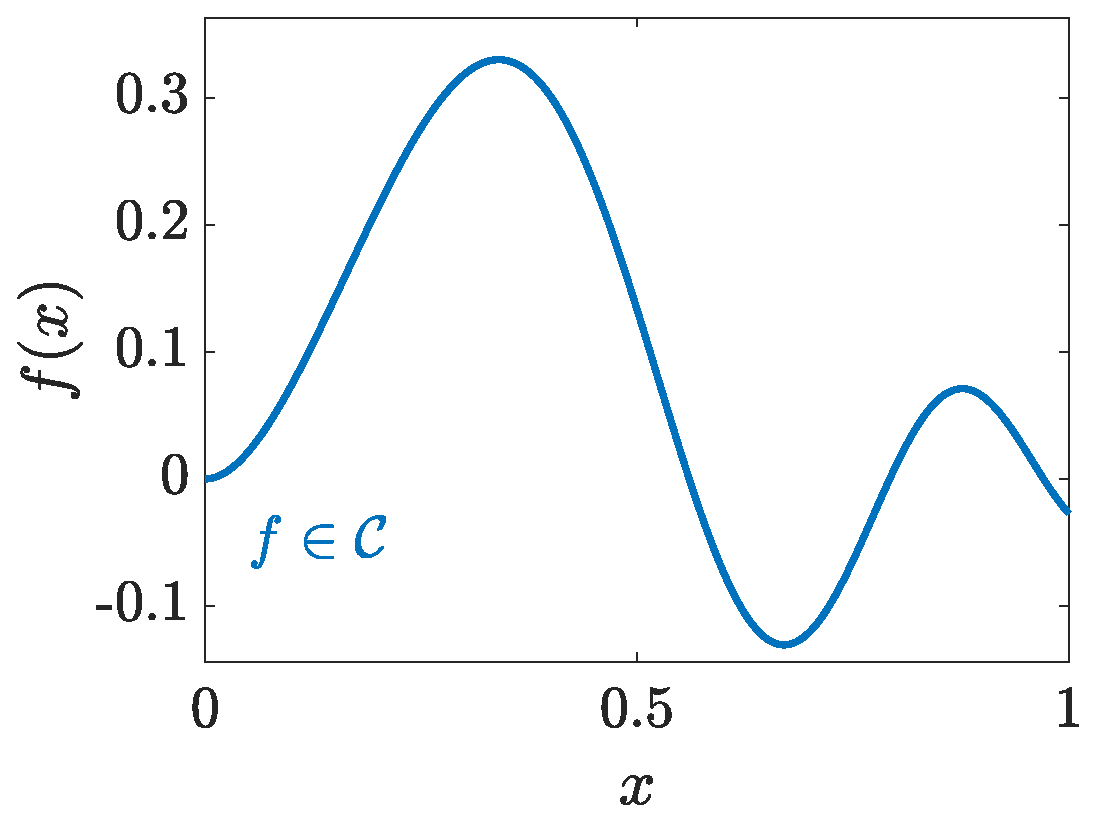
\includegraphics[width = \figwidth] 
	{ProgramsImages/FunctionWalshFourierCoeffDecay.eps} \qquad \qquad
	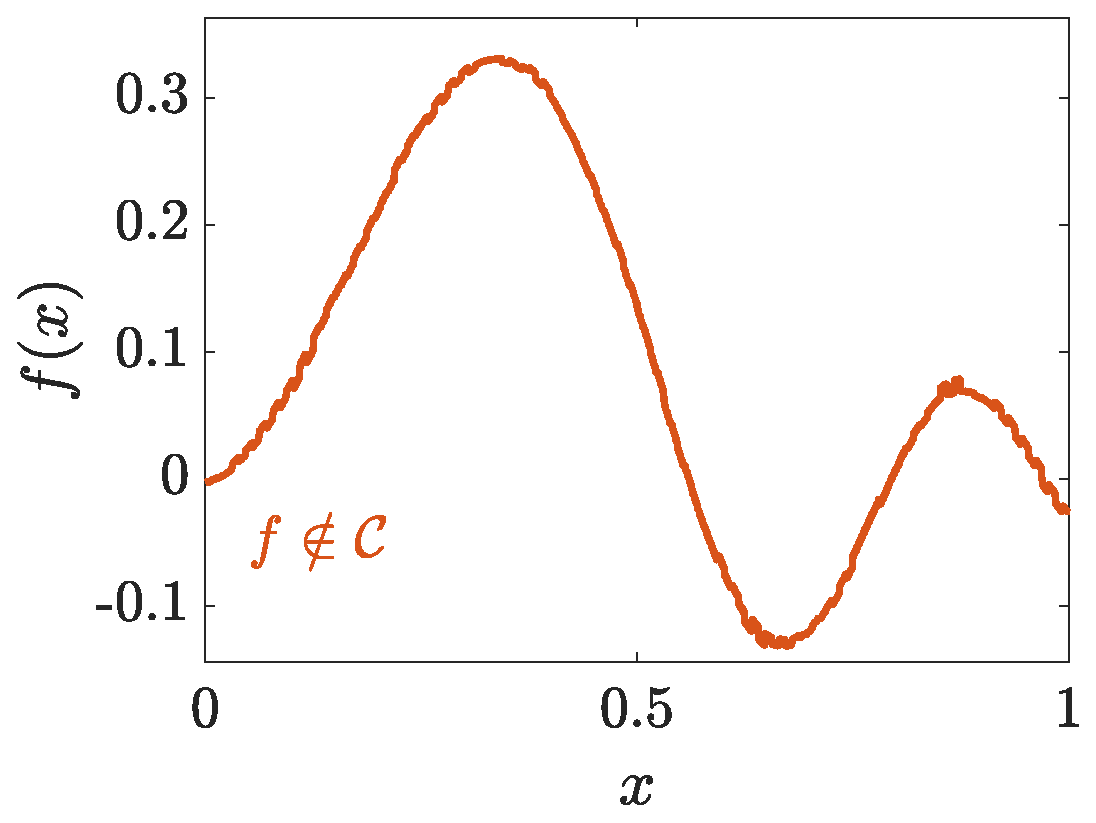
\includegraphics[width = \figwidth] 
	{ProgramsImages/FilteredFunctionWalshFourierCoeffDecay.eps} }


\end{frame}


\begin{frame}{ Option Pricing\footfullcite{ChoEtal17b}}
\vspace{-12ex}
\begin{tabular}{m{11cm}m{2.5cm}}
	\[
	\begin{aligned}
	 \text{fair price} = 
	\int_{\reals^d}\me^{-r T}\max\left(\frac{1}{d}\sum_{j=1}^d S_{j}-K, 0\right) 
	\frac{\me^{-\vz^T\vz/2}}{(2\pi)^{d/2}}\,\dif \vz \approx \$13.12
	\end{aligned}
	\]
	& 
	\financePict
\end{tabular}
\vspace{-4ex}
\begin{gather*}
S_{j} =  S_0\me^{(r-\sigma^2/2)jT/d+\sigma x_j} = \text{stock price at time } 
jT/d, \\
\vx  = \mA \vz, \quad \mA \mA^T = \mSigma = \Bigl ( \min(i,j) T/d \Bigr) _{i,j = 1}^d,
\quad T = 1/4, \ d=13 \text{ here}
\end{gather*}
\begin{equation*}
\begin{array}{cccccccc}
\text{Error}& && \text{Median}&& \text{Worst 10\%} & \text{Worst 10\%} \\
\text{Tolerance} & \multicolumn{2}{c}{\text{Method}}  & \text{Error} & \text{Accuracy} 
& n & \text{Time (s)} \\
\toprule
\input{ProgramsImages/AsianOutput.txt}
\end{array}
\end{equation*}
\vspace{-8ex}

\end{frame}


\section{General Linear Problems}

\begin{frame}{Solving General Linear Problems Using Series Coefficients, $\LambdaSer$\footfullcite{DinHic20a}}

\vspace{-7ex}

\begin{align*}
    \only<1>{\cf &:= \left \{ f = \sum_{\vj \in \cn} \hf(\vj) u_{\vj} : \norm[\cf]{f} := \norm[2]{\left(\frac{\bigabs{\hf(\vj)}}{\lambda_{\vj}} \right)_{\vj \in \cn}} \right \} \qquad \begin{minipage}{3cm}\raggedright\alert{$\vlambda$ affects convergence rate \& tractability}\end{minipage}\\
    \cg &: = \biggl \{ g = \sum_{\vj \in \cn} \hg(\vj) v_{\vj} : \norm[\cg]{g} := \bignorm[2]{\hg}\biggr \}, \qquad v_{\vj} = S(u_{\vj}) \\[-2ex]}
      & \alert{\lambda_{\vj_1} \ge \lambda_{\vj_2} \ge \cdots}, \qquad
      n_0 < n_1 < n_2 < \cdots,  \qquad
 	\sigma_k(f) = \sqrt{\sum_{i=n_{k-1}+1}^{n_k}  \bigabs{\hf(\vj_i)}^2}, \quad k \in \naturals \\
     \cc &: = \left\{f \in \cf :  
 	 \sigma_\ell(f) \le a b^{\ell - k}\sigma_k(f) \quad \forall k \le \ell \right\} \quad a > 1 > b \quad \text{\alert{series coef.\ decay steadily}}\\
 	 \Sapp(f,n_k) &= \sum_{i=1}^{n_k} \hf(\vj_i) v_{\vj_i} \text{ is optimal for fixed }n_k, \qquad \norm[\cg]{S(f) - \Sapp(f,n_k)} \le \frac{ab \sigma_k(f)}{\sqrt{1 - b^2}} \\[-1ex]
 	 \alert{A(f,\varepsilon)} & \alert{= \Sapp(f,n_k)} \text{ for the smallest $k$ satisfying } \alert{\sigma_k(f) \le \frac{\varepsilon \sqrt{1 - b^2}}{ab}}
 	 \only<2>{\\ 
 	 \MoveEqLeft{\alert{\cost(A,\cc,\varepsilon,\rho) = n_{\ell^\dagger}}, \quad 
 	 \ell^\dagger \le \min \left \{\ell \in \naturals : \frac{\rho^2}{\varepsilon^2} \le \frac{(1 - b^2)}{a^2b^2} \left[ \sum_{k=1}^{\ell-1} \frac{b^{2(k-\ell)}}{a^2\lambda_{n_{k-1}+1}^2} + \frac{1}{\lambda_{n_{\ell-1}+1}^2}\right]   \right\}} \\
 	 \MoveEqLeft{\cost(A,\cc,\varepsilon,\rho) \text{ \alert{essentially no worse than} } \comp(\ca(\cc,\LambdaAll),\varepsilon,\rho)}\\
 	 \MoveEqLeft{\text{\alert{No} tractability results}}}
\end{align*}

\end{frame}

\section{Function Approximation}

\begin{frame}{\emph{Function Approximation} when Function Values Are Expensive\footfullcite{WuHam00,KuoEtal12a}}

\vspace{-7ex}

    \begin{align*}
    \only<1>{\cf &:= \left \{ f = \sum_{\vj \in \natzero^d} \hf(\vj) u_{\vj} : \norm[\cf]{f} :=  \norm[\infty]{\left(\frac{\bigabs{\hf(\vj)}}{\lambda_{\vj}} \right)_{\vj \in \cn}} \right \} \qquad \begin{minipage}{3cm}\raggedright\alert{$\vlambda$ affects convergence rate \& tractability}\end{minipage}\\
    \cg &: = \Biggl \{ g = \sum_{\vj \in \natzero^d} \hg(\vj) v_{\vj} : \norm[\cg]{g} := \bignorm[1]{\hg}\Biggr \}, \qquad v_{\vj} = S(u_{\vj}) = u_{\vj} \\[-2ex]}
    \lambda_{\vj} & = \Gamma_{\norm[0]{\vj}} \prod_{\substack{\ell = 1 \\ j_{\ell} > 0}}^d \gamma_\ell s_{j_\ell} \quad
    \begin{cases}
\gamma_\ell = \text{coordinate importance} \\[-0.5ex]
\Gamma_r = \text{order size} \\[-0.5ex]
s_j =  \text{smoothness degree}
\end{cases} \quad\begin{minipage}{5.5cm}\raggedright\alert{POSD weights reflect effect sparsity, effect hierarchy, effect heredity, and effect smoothness}\end{minipage}
 \\[-2ex]
      & \alert{\lambda_{\vj_1} \ge \lambda_{\vj_2} \ge \cdots}, \qquad
      \Sapp(f,n) = \sum_{i=1}^{n} \hf(\vj_i) u_{\vj_i} ,  \qquad
 	\norm[\cg]{S(f) - \Sapp(f,n_k)} \le \norm[\cf]{f} \sum_{i = n+1} \lambda_{\vj_i} \\
     \cc &: = \left\{f \in \cf :  \text{ those functions for which } \norm[\cf]{f} \text{ can be \alert{inferred} from a pilot sample} \right \}
\end{align*}

\end{frame}

\begin{frame}{Legendre and Chebyshev Bases for Function Approximation}
\vspace{-3ex}
	\begin{tabular}{>{\centering}m{0.18\textwidth}>{\centering}m{0.18\textwidth}>{\centering}m{0.18\textwidth}>{\centering}m{0.18\textwidth}>{\centering}m{0.18\textwidth}}
		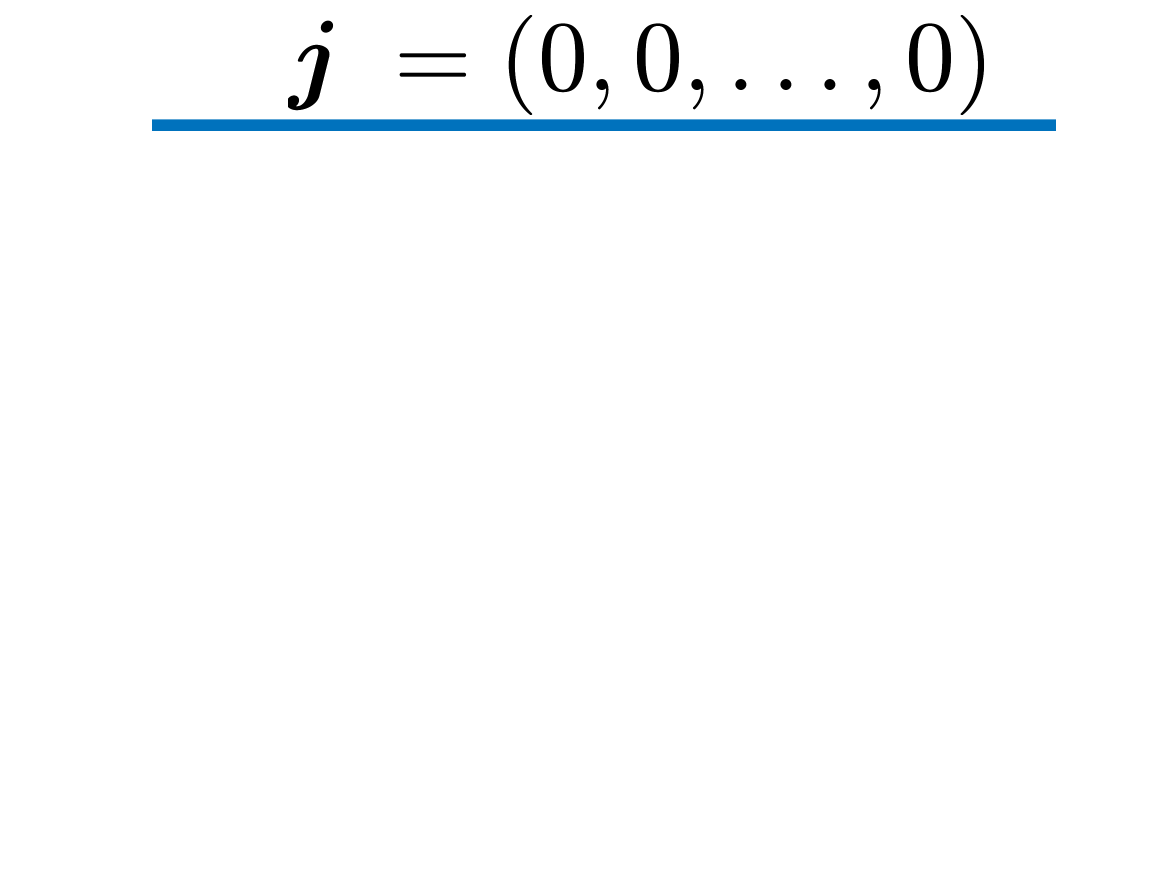
\includegraphics[width =0.18\textwidth]{ProgramsImages/Legendre_Degree_0.png}  &
		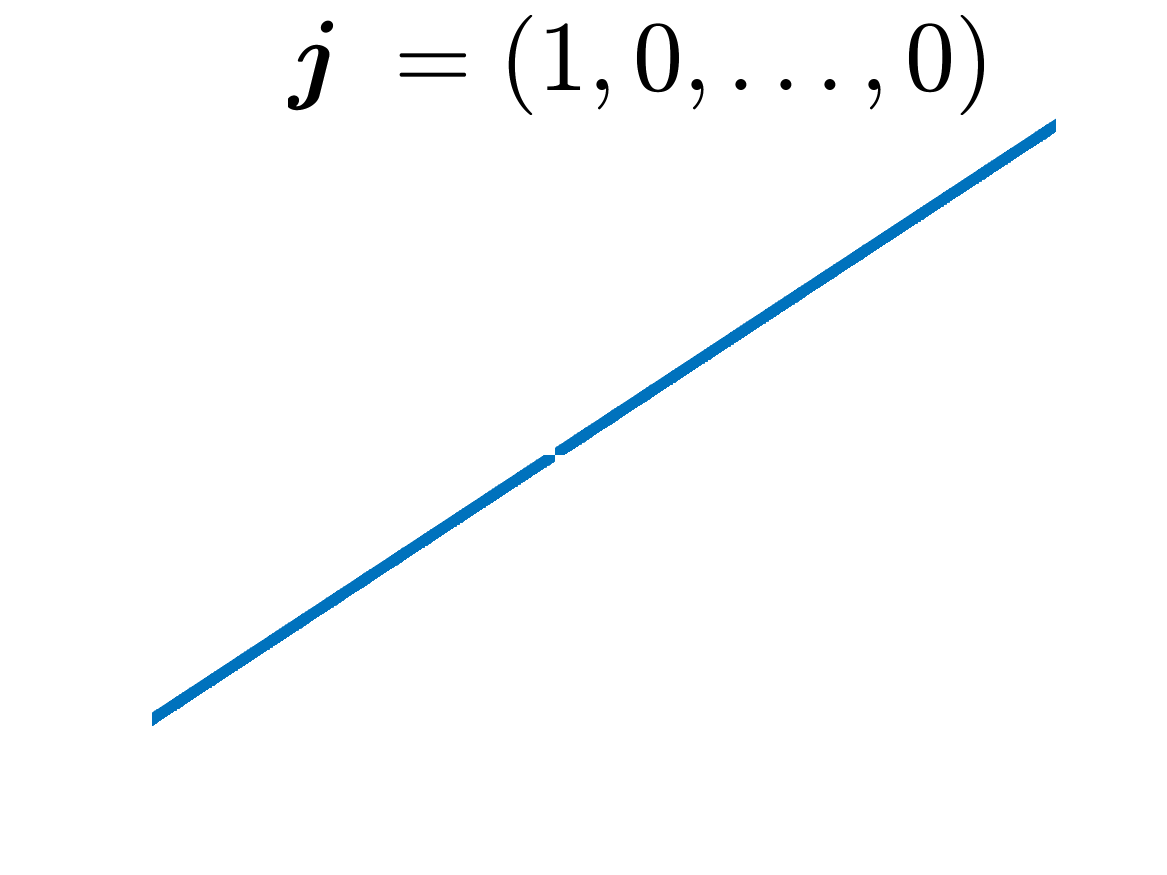
\includegraphics[width =0.18\textwidth]{ProgramsImages/Legendre_Degree_1.png}  &
		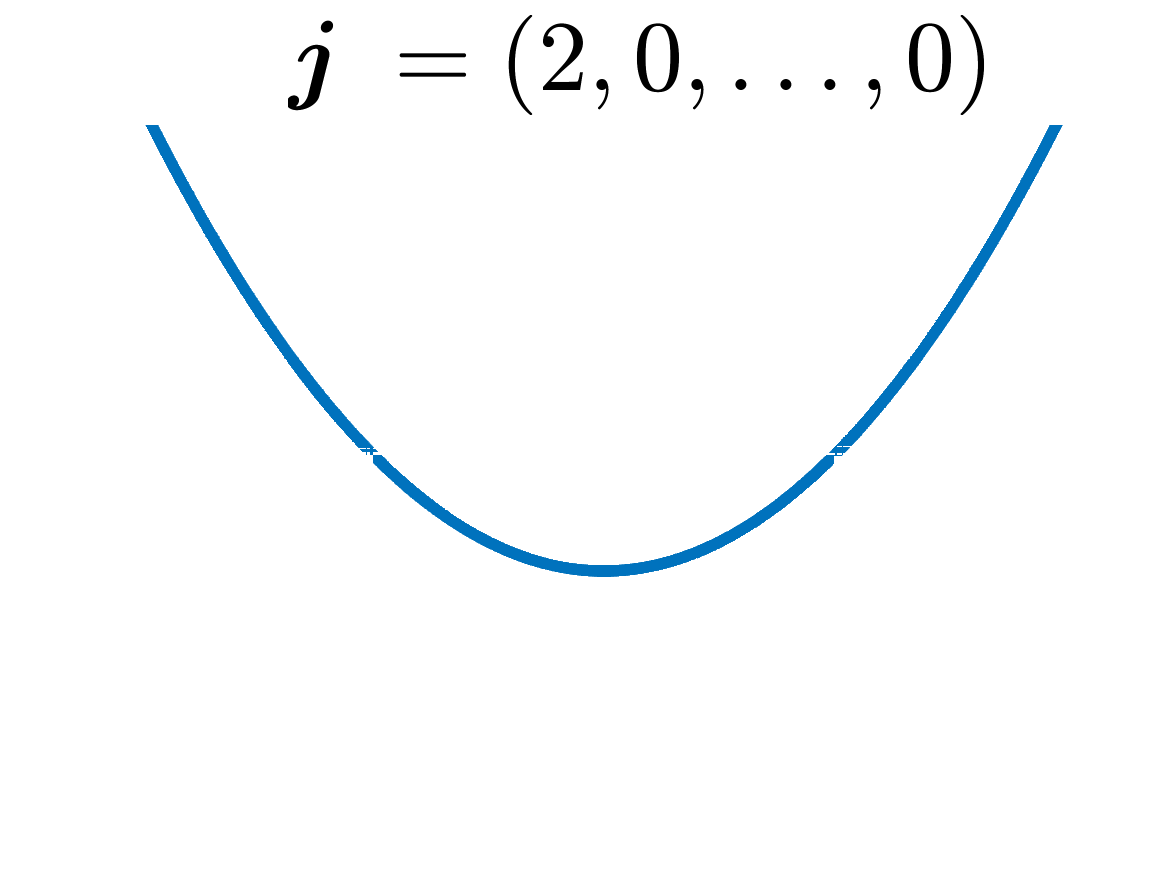
\includegraphics[width =0.18\textwidth]{ProgramsImages/Legendre_Degree_2.png}  &
		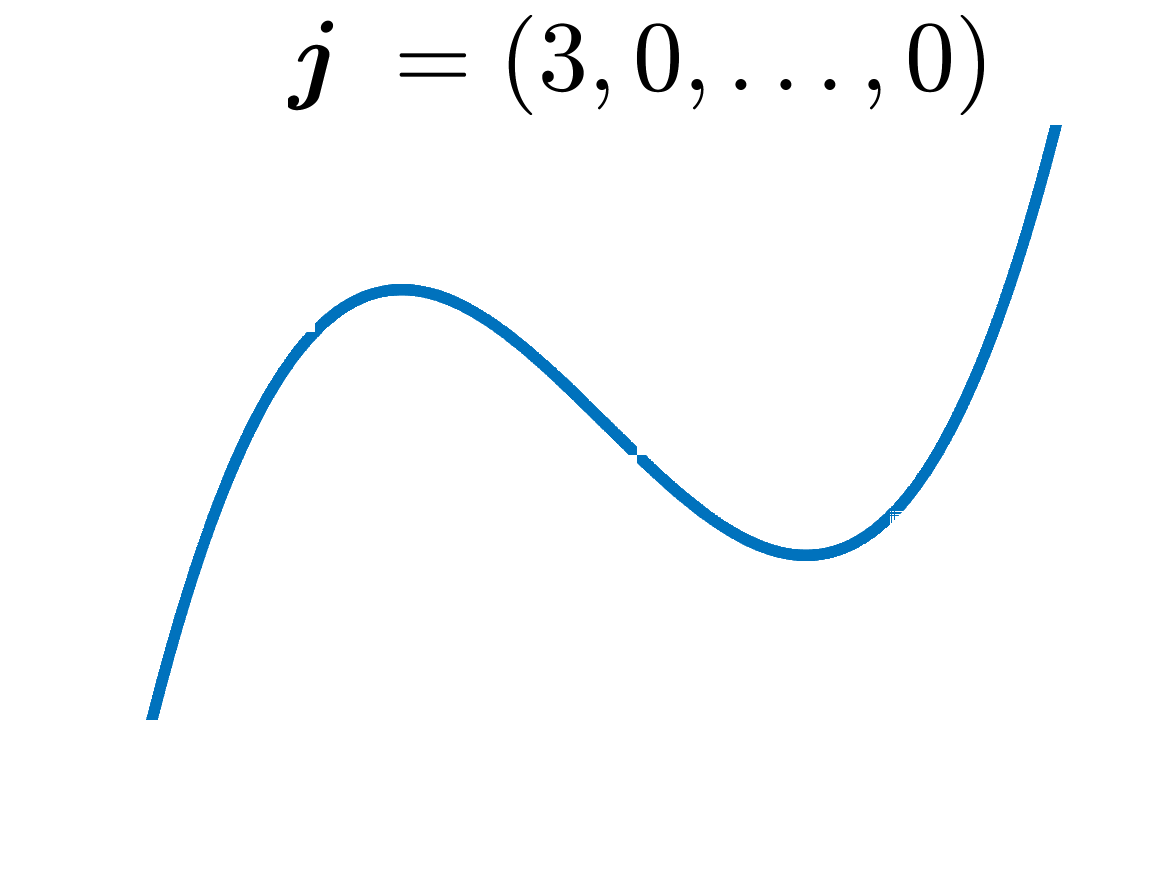
\includegraphics[width =0.18\textwidth]{ProgramsImages/Legendre_Degree_3.png}  &
		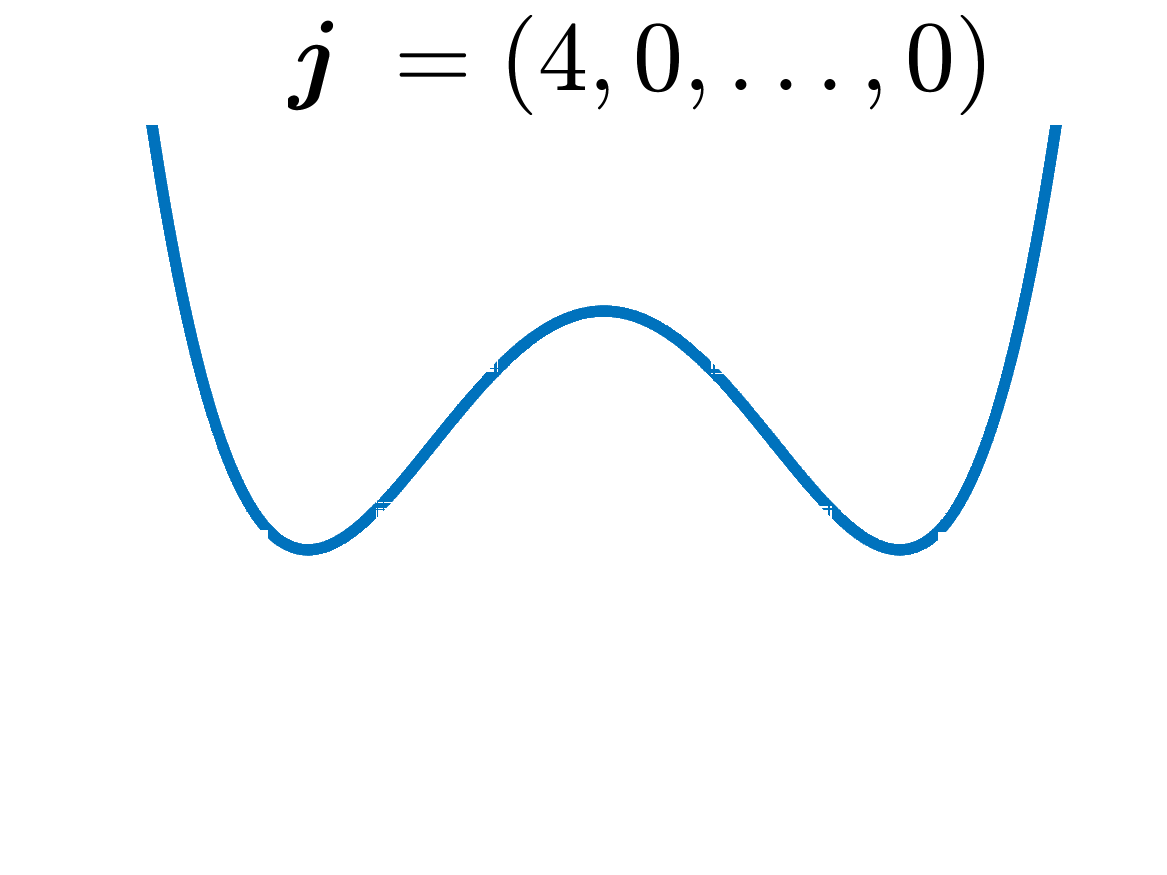
\includegraphics[width =0.18\textwidth]{ProgramsImages/Legendre_Degree_4.png} 
	\tabularnewline[-7ex]
	Legendre
	\tabularnewline
	\tabularnewline
		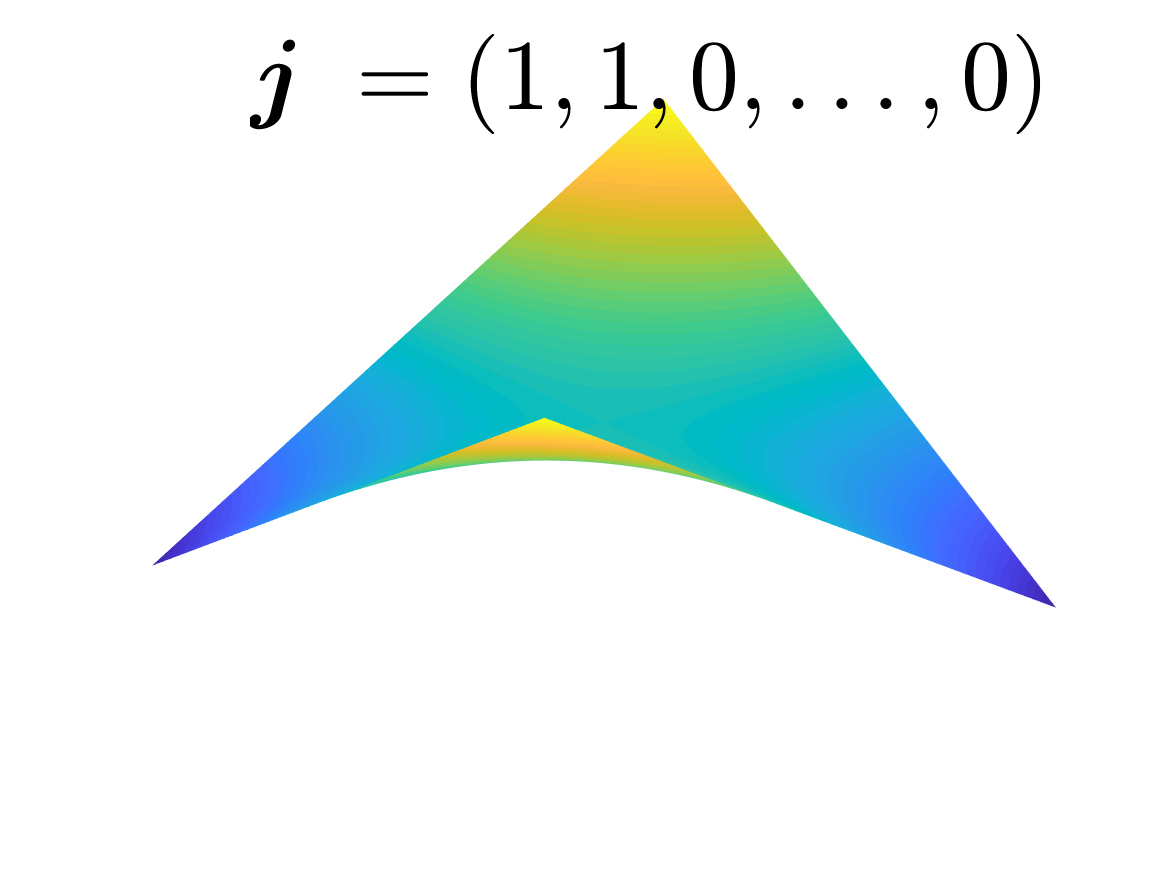
\includegraphics[width =0.18\textwidth]{ProgramsImages/Legendre_Degree_1_1.png}  &
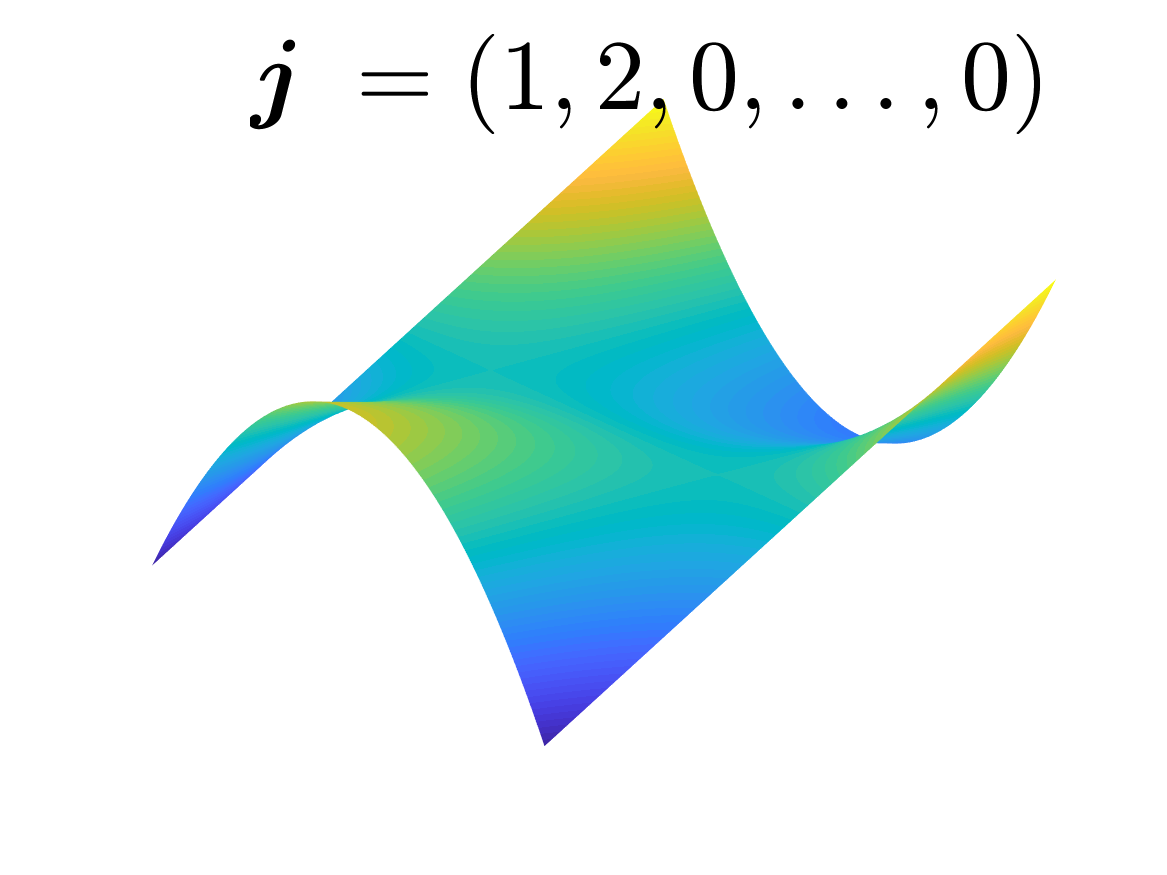
\includegraphics[width =0.18\textwidth]{ProgramsImages/Legendre_Degree_1_2.png}  &
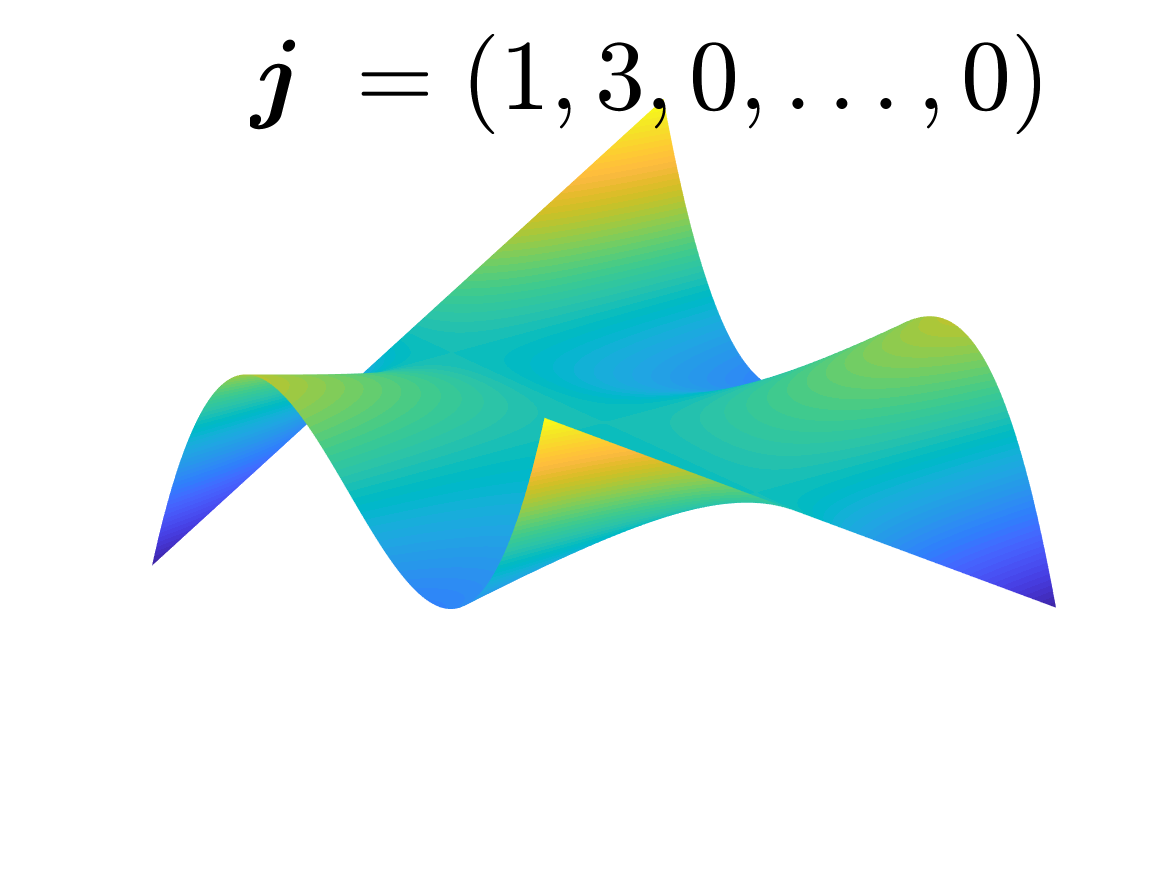
\includegraphics[width =0.18\textwidth]{ProgramsImages/Legendre_Degree_1_3.png}  &
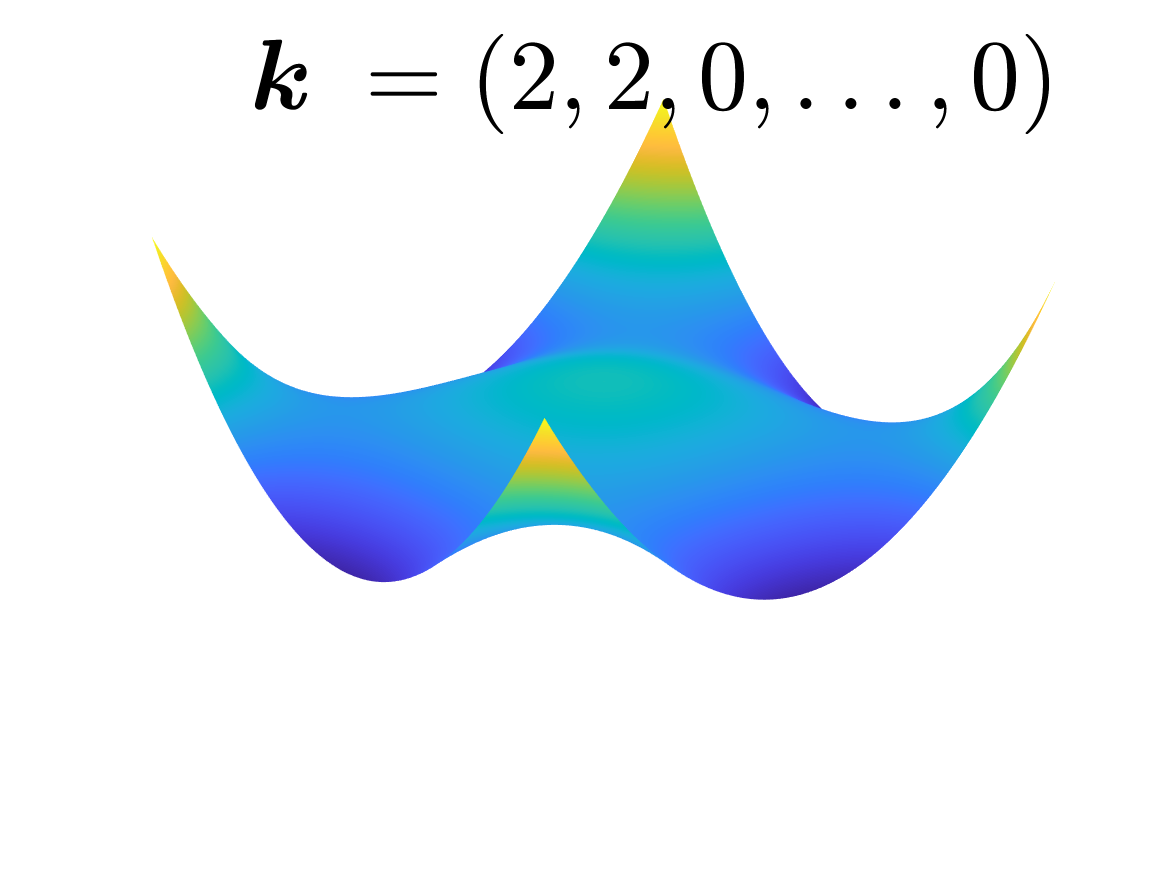
\includegraphics[width =0.18\textwidth]{ProgramsImages/Legendre_Degree_2_2.png}  &
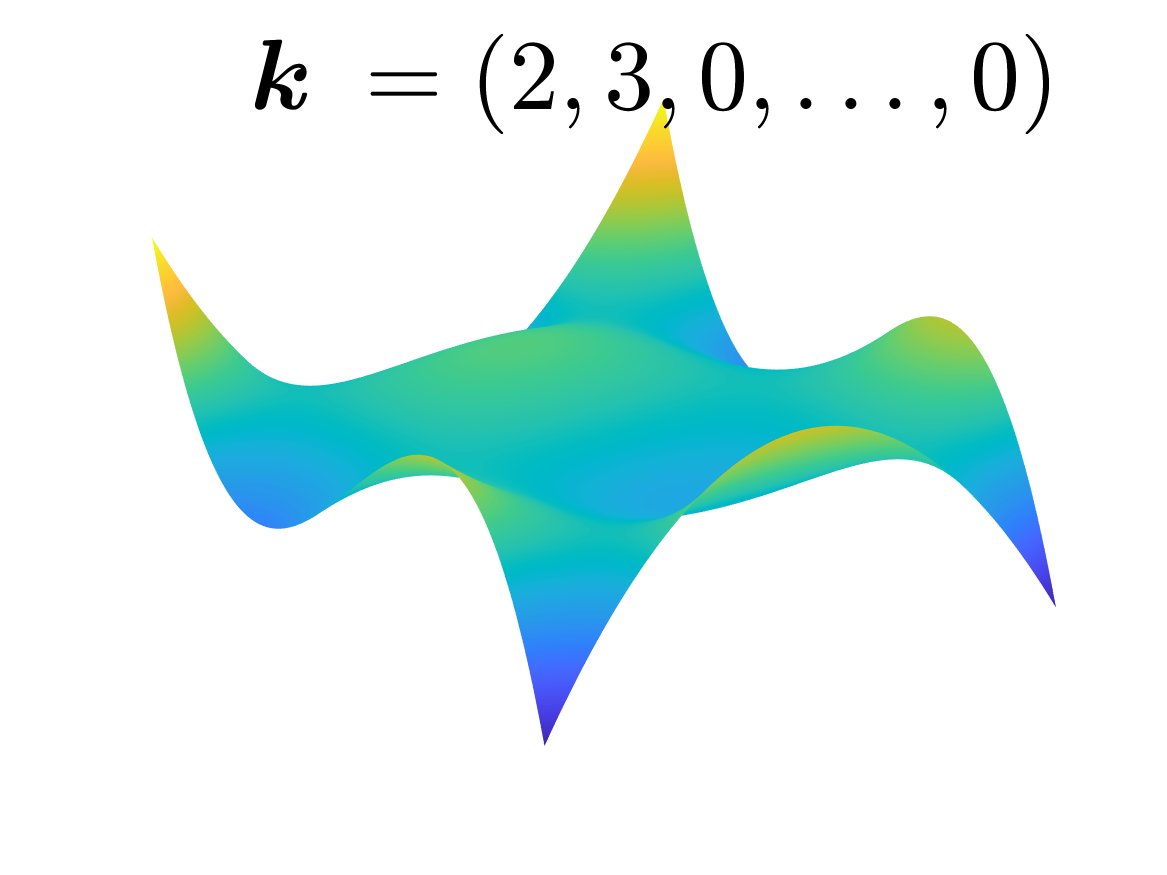
\includegraphics[width =0.18\textwidth]{ProgramsImages/Legendre_Degree_2_3.png} 
\tabularnewline[0ex]
		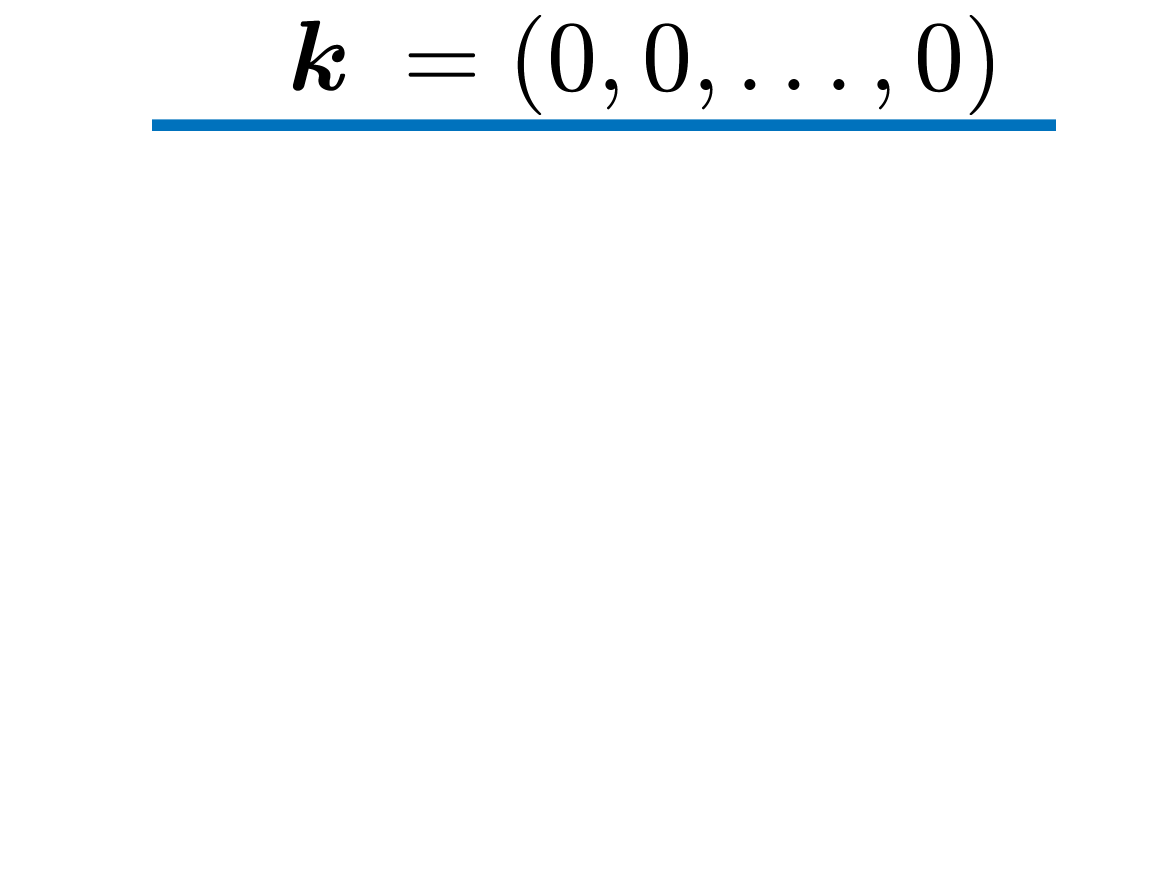
\includegraphics[width =0.18\textwidth]{ProgramsImages/Chebyshev_Degree_0.png}  &
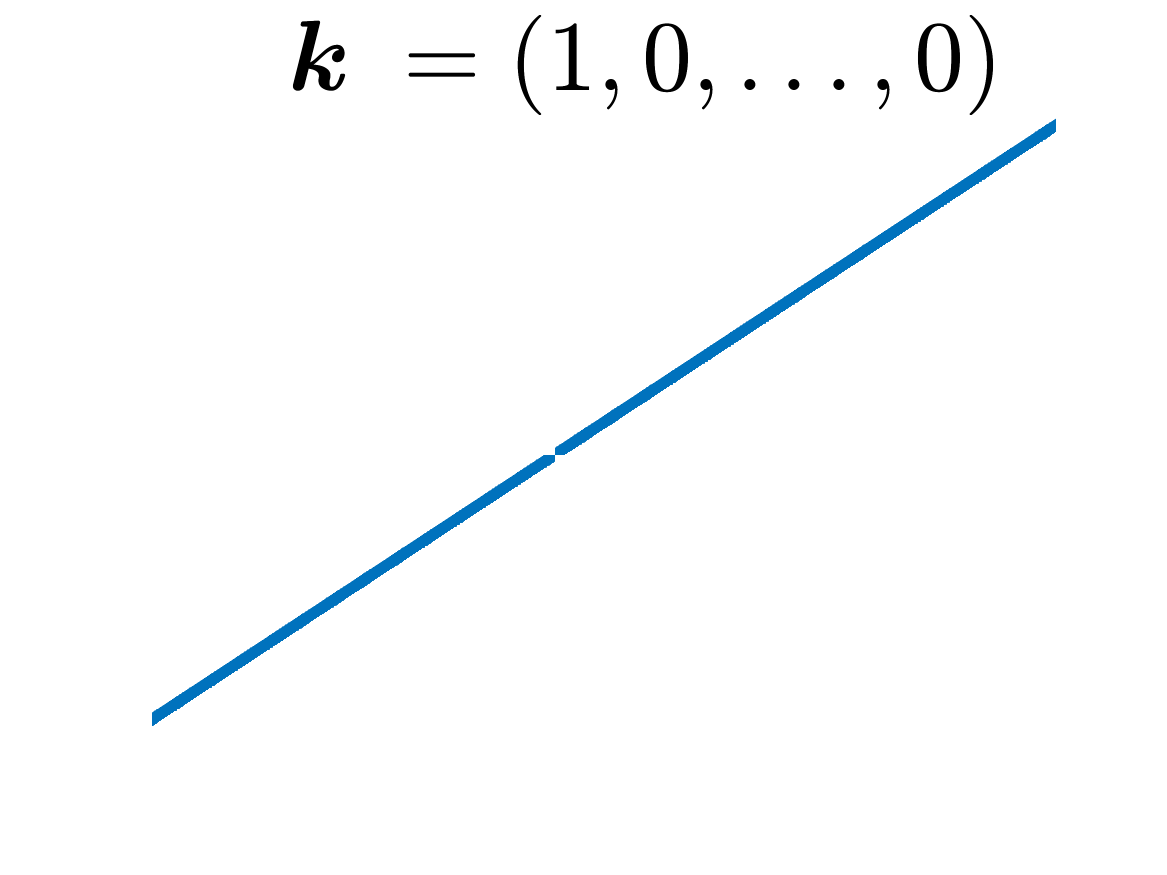
\includegraphics[width =0.18\textwidth]{ProgramsImages/Chebyshev_Degree_1.png}  &
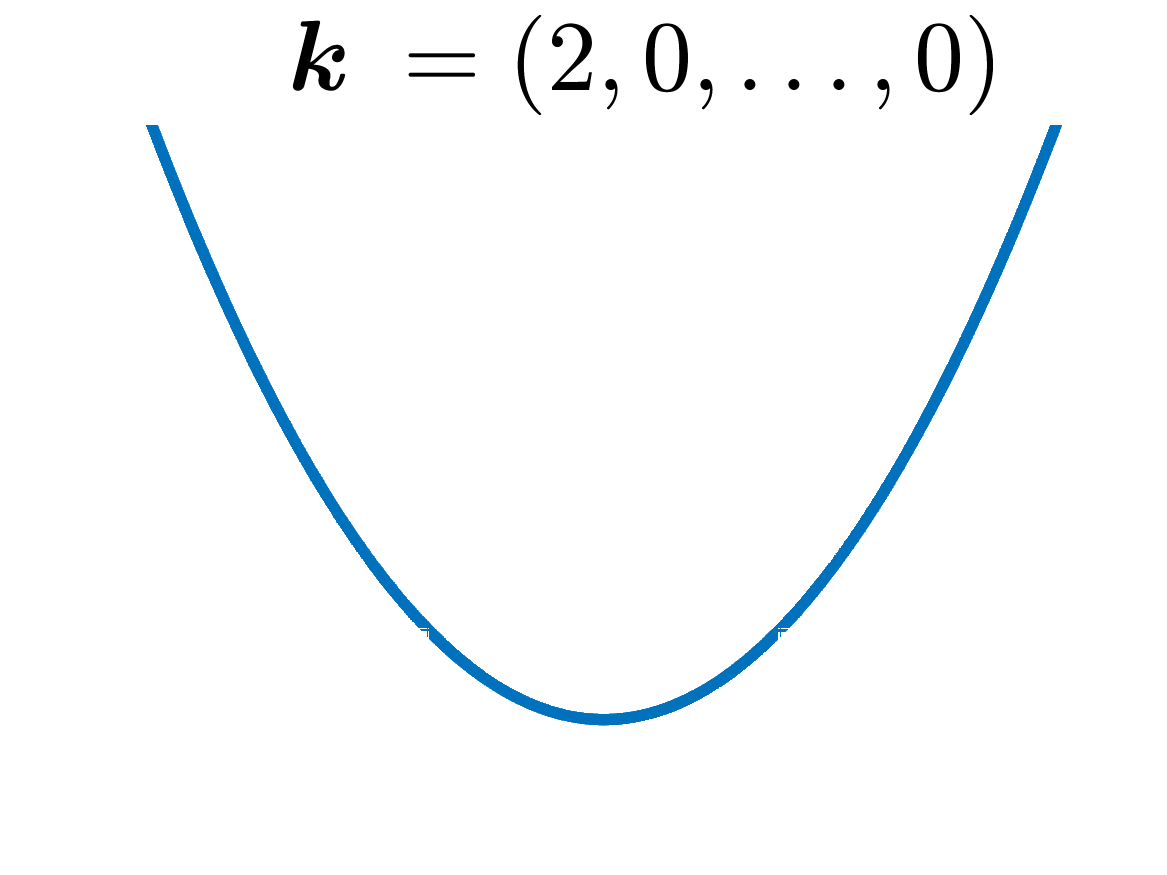
\includegraphics[width =0.18\textwidth]{ProgramsImages/Chebyshev_Degree_2.png}  &
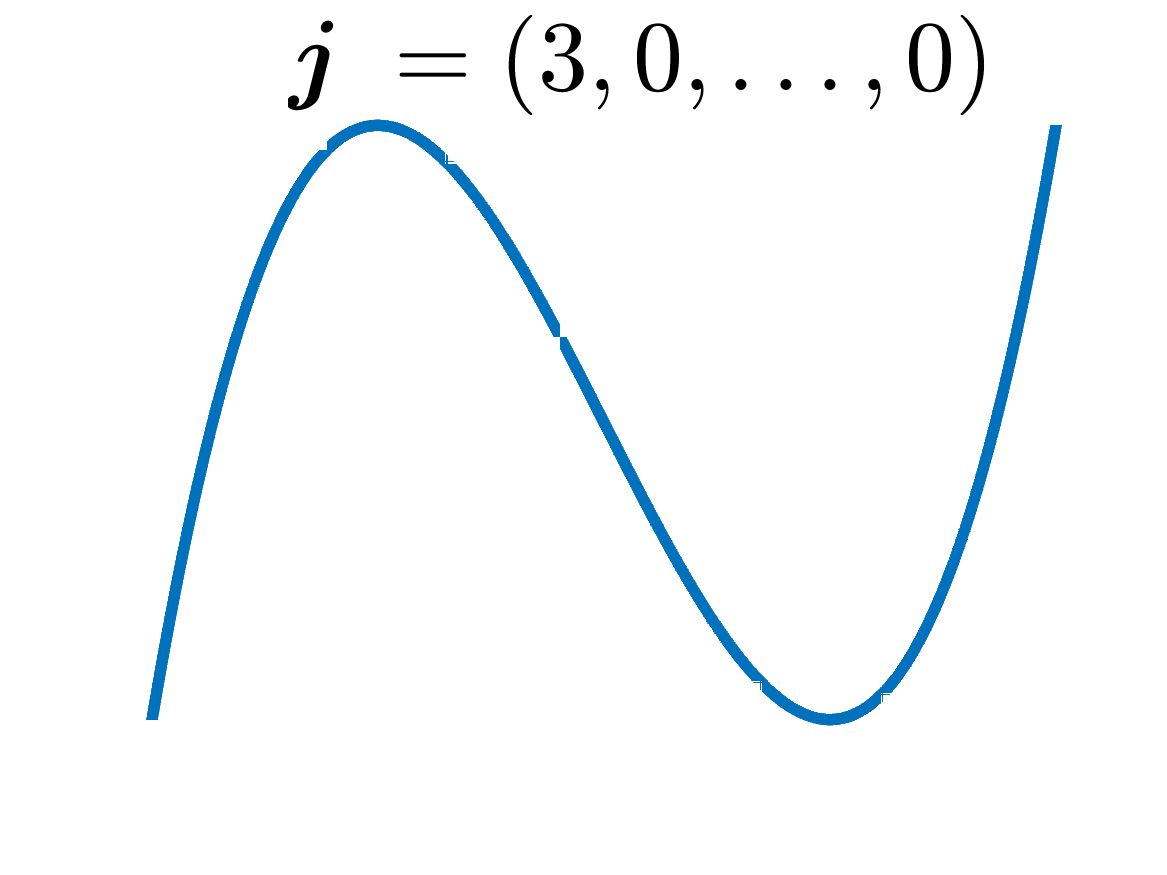
\includegraphics[width =0.18\textwidth]{ProgramsImages/Chebyshev_Degree_3.png}  &
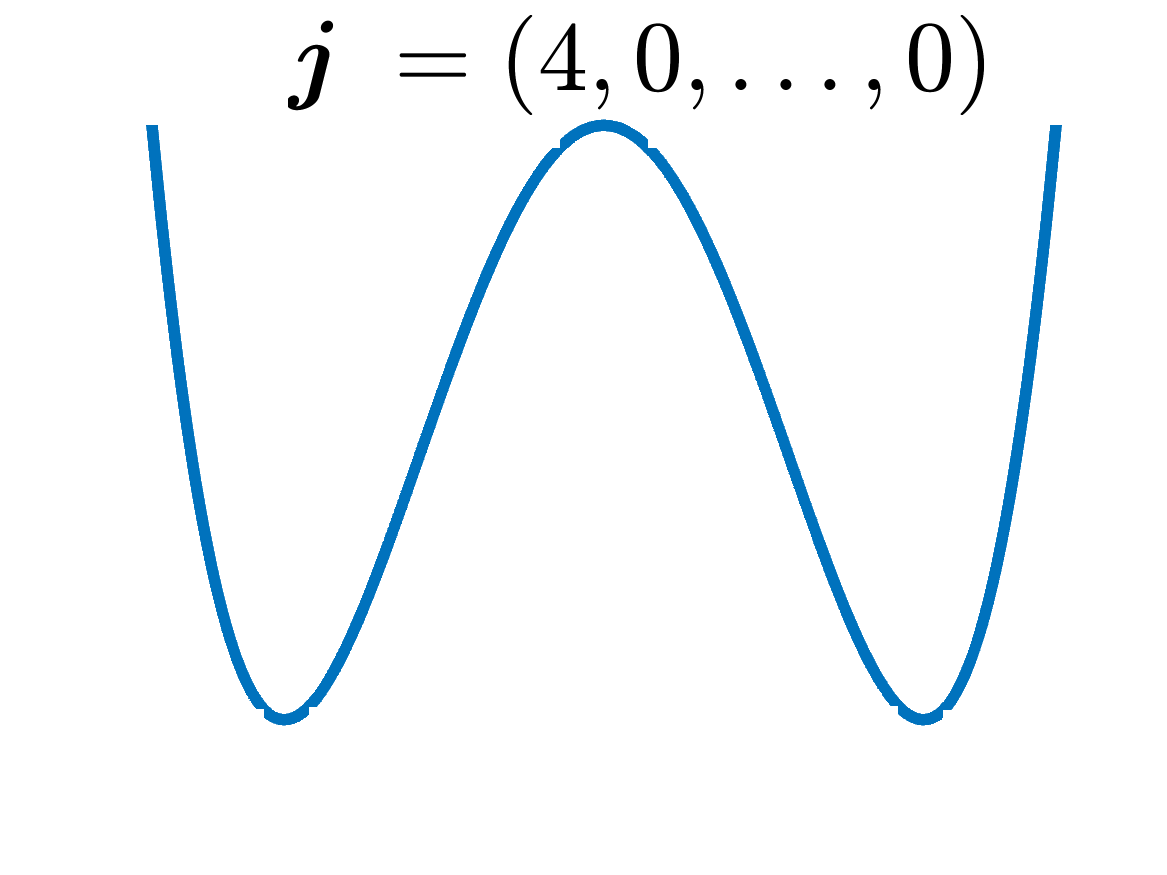
\includegraphics[width =0.18\textwidth]{ProgramsImages/Chebyshev_Degree_4.png} 
\tabularnewline[-7ex]
Chebyshev \tabularnewline
\tabularnewline
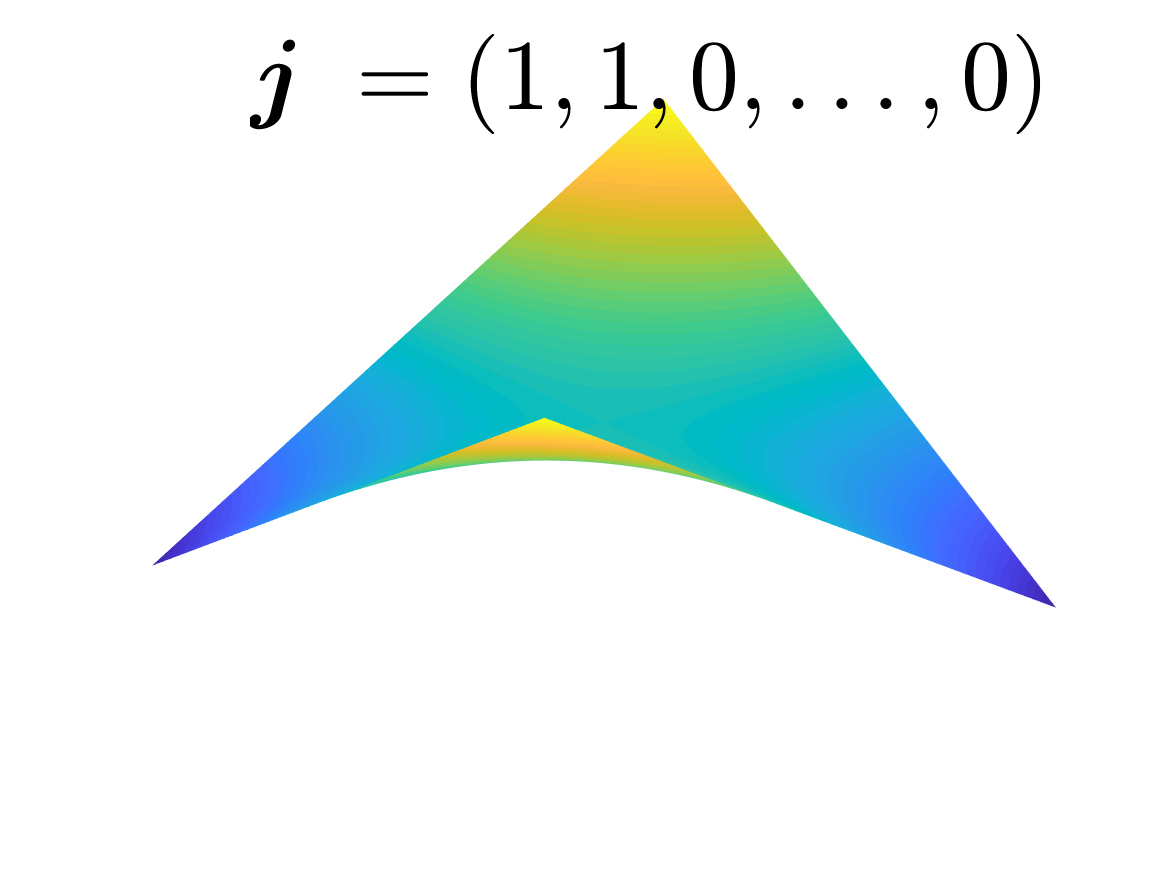
\includegraphics[width =0.18\textwidth]{ProgramsImages/Chebyshev_Degree_1_1.png}  &
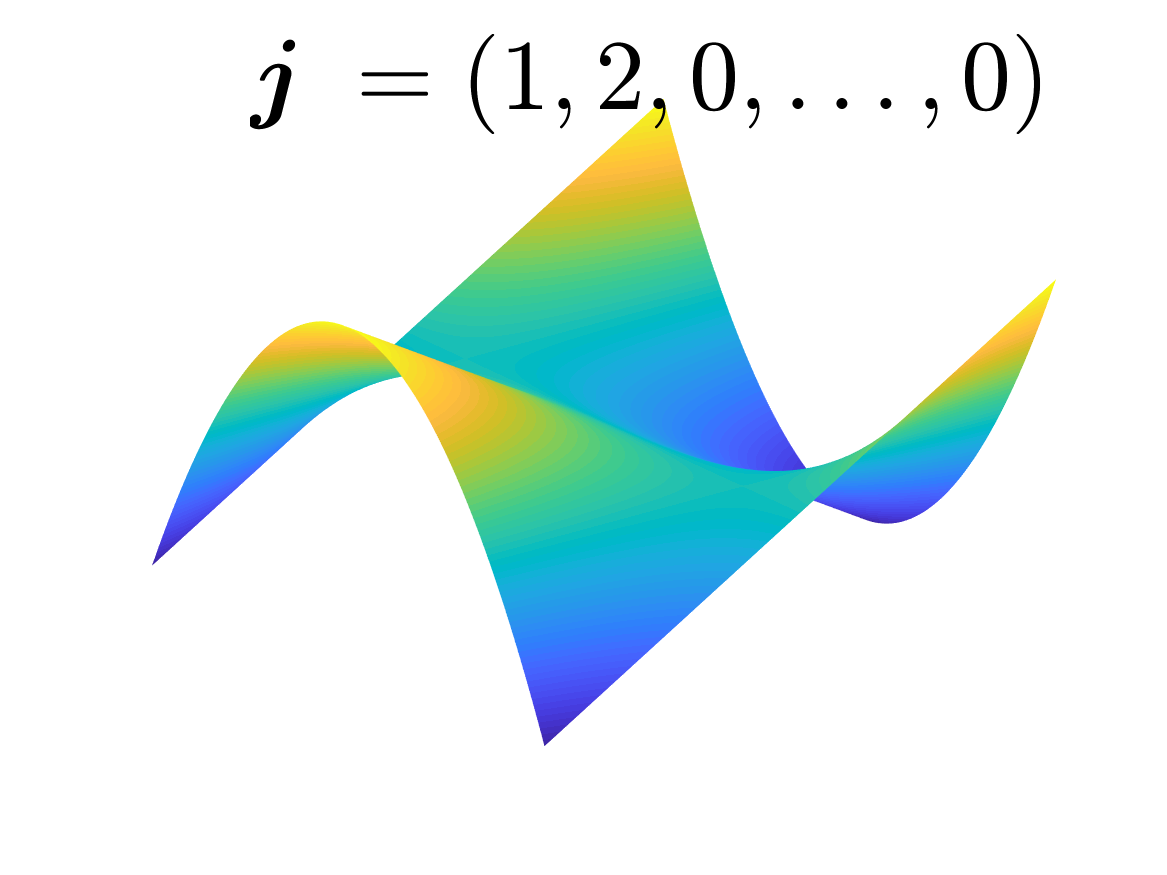
\includegraphics[width =0.18\textwidth]{ProgramsImages/Chebyshev_Degree_1_2.png}  &
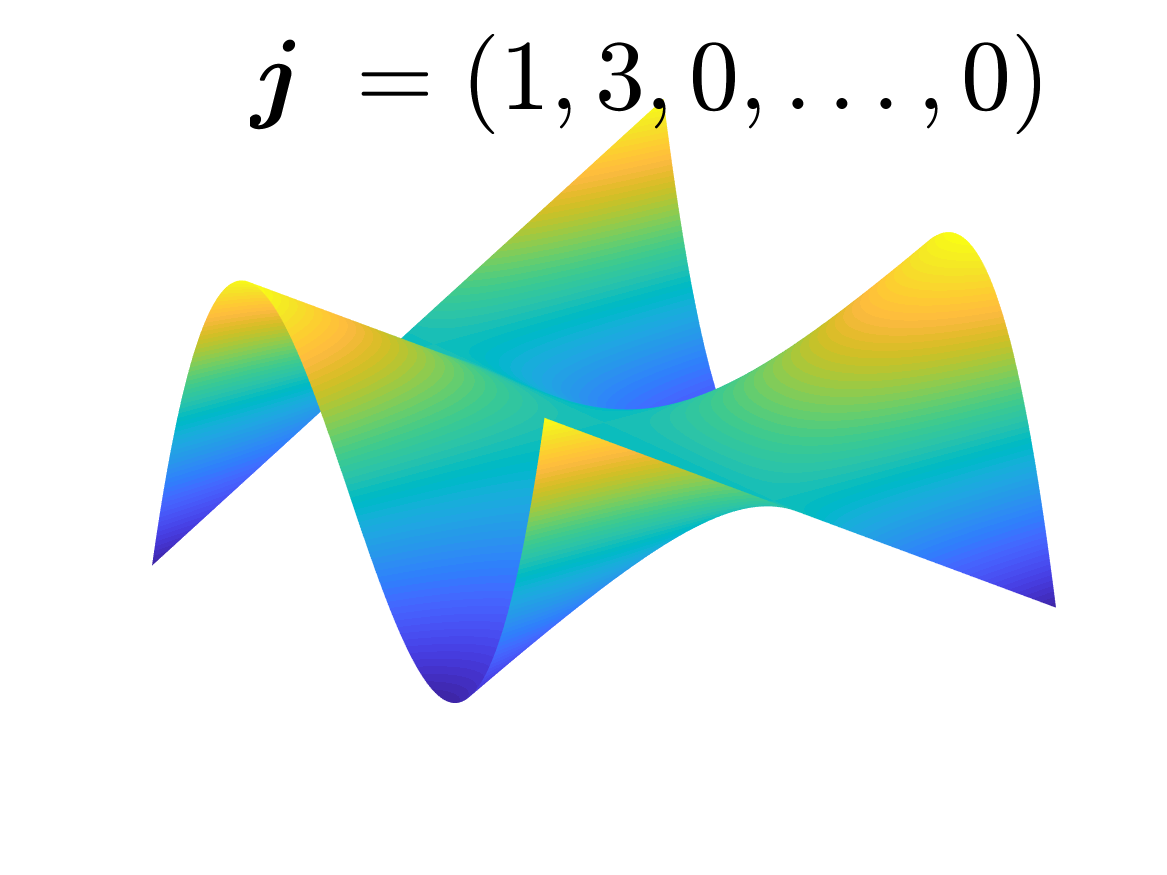
\includegraphics[width =0.18\textwidth]{ProgramsImages/Chebyshev_Degree_1_3.png}  &
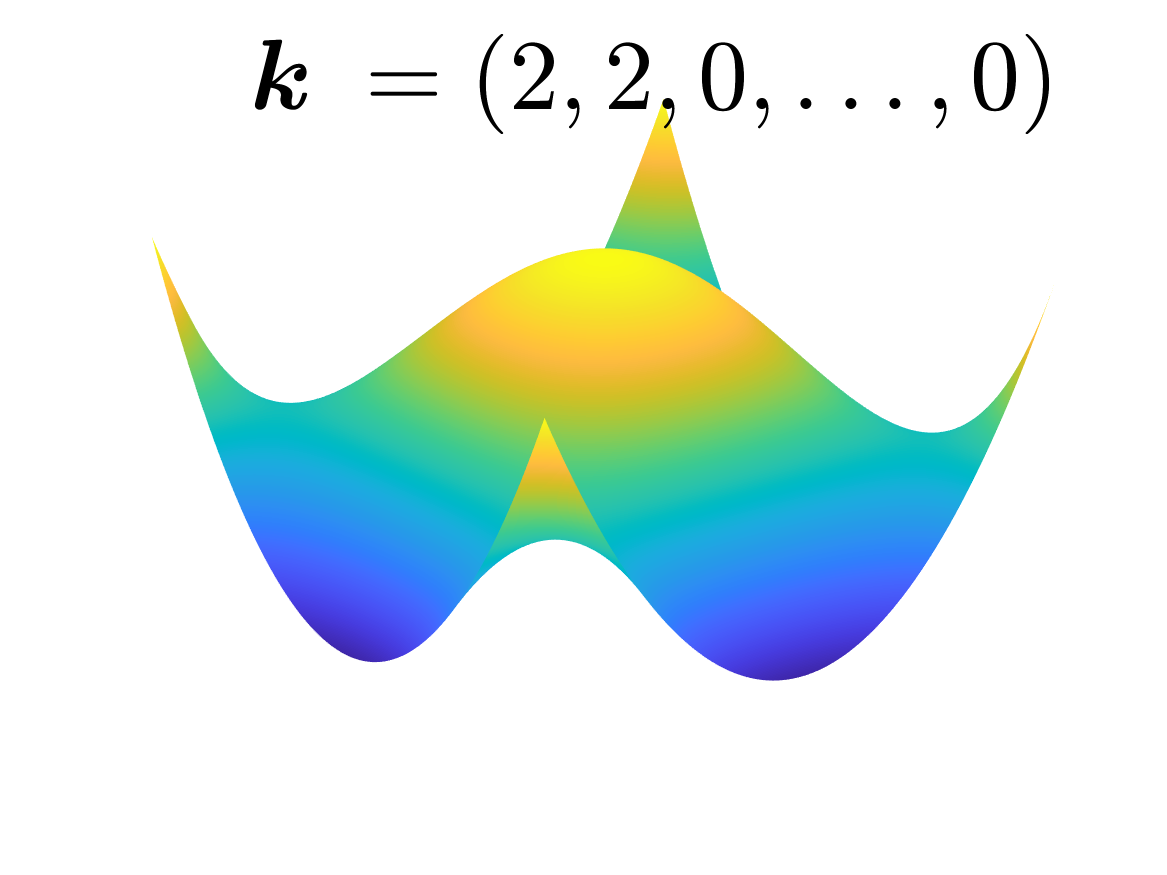
\includegraphics[width =0.18\textwidth]{ProgramsImages/Chebyshev_Degree_2_2.png}  &
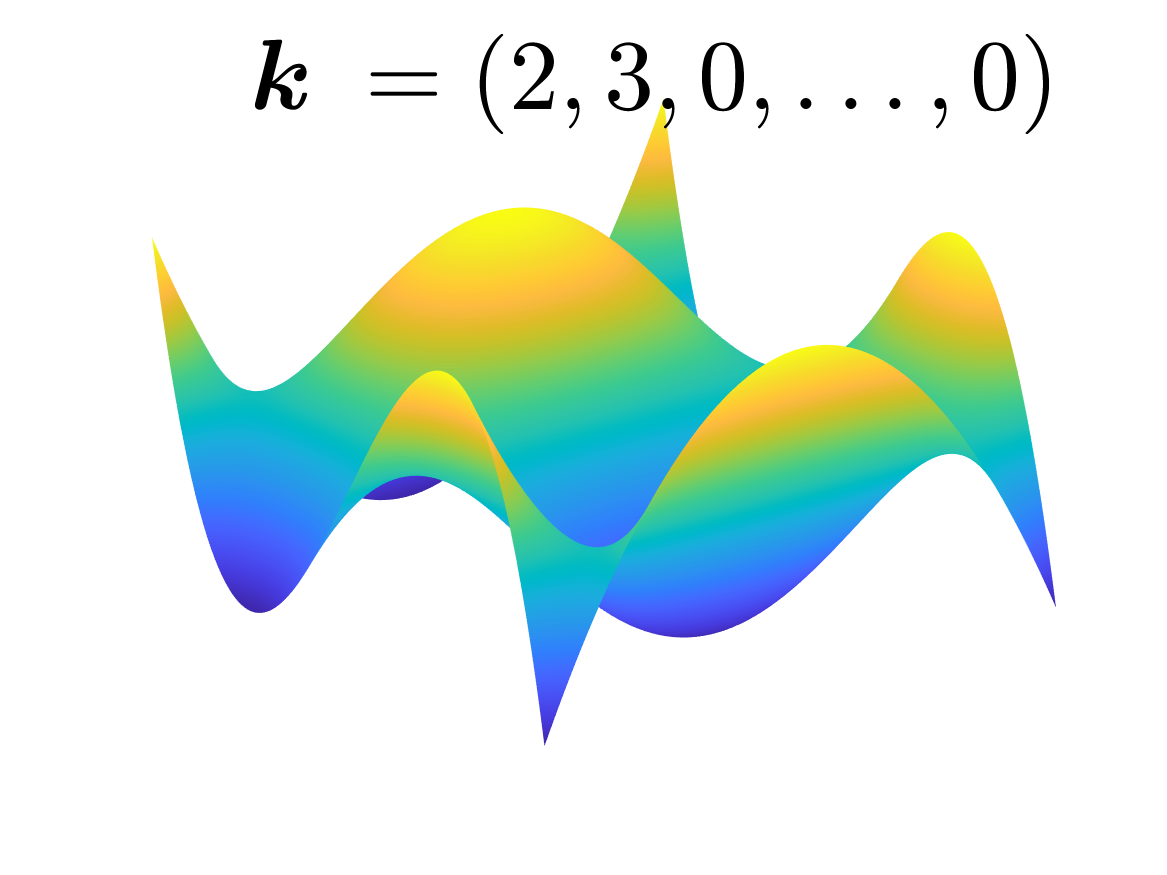
\includegraphics[width =0.18\textwidth]{ProgramsImages/Chebyshev_Degree_2_3.png} 
	\end{tabular}
\end{frame}

\begin{frame}{Cheng and Sandu Function\footfullcite{VirLib17a}}
    \vspace{-9ex}
    \begin{gather*}
        \text{Chebyshev polynomials}, \qquad \text{Order weights }\Gamma_k = 1, \qquad \text{Coordinate weights } \gamma_\ell \text{ \alert{inferred}}, \\
        \text{Smoothness weights } s_j \text{ \alert{inferred}}, \qquad \LambdaStd
    \end{gather*}
    
    \vspace{-3ex}
    
    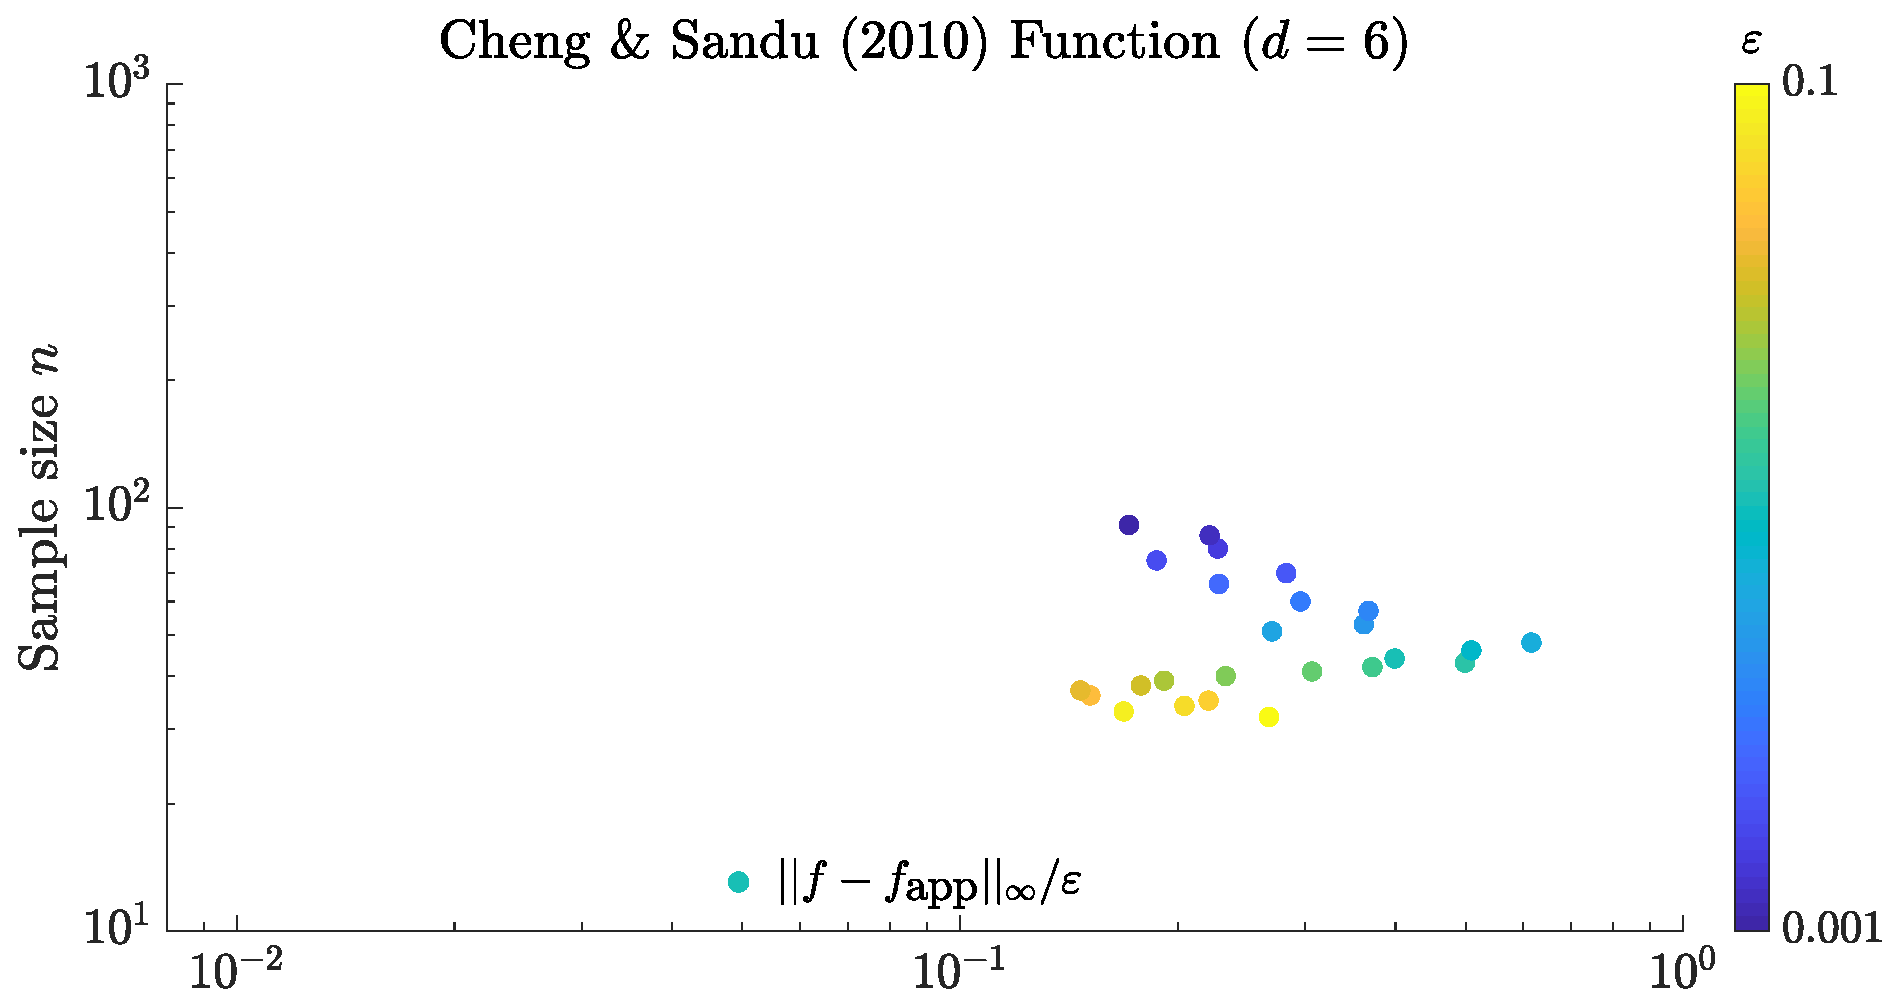
\includegraphics[height = 4.3cm]{ProgramsImages/sim_eval_results_chsan10_d6_sflg0ErrN.eps}
    \qquad \includegraphics[height = 4.3cm]{ProgramsImages/sim_eval_results_chsan10_d6_sflg0fErr.eps}
\end{frame}


\section{Summary}
\begin{frame}{Take Home Messages}

\vspace{-4ex}

\begin{itemize}
    \item Assuming that the input functions lie in convex \alert{cones} \smallcone allow us to construct \alert{adaptive} algorithms
    
    \item Cone definitions reflect \alert{prior beliefs} and/or \alert{practical considerations}
    
    \item Demonstration of concept
    \begin{itemize}
        \item Integration using $\LambdaStd$
        \begin{itemize}
            \item Constructed $A \in \ca(\cc,\LambdaStd)$
            \item No cost, complexity, or tractability yet
        \end{itemize}
        \item General linear problems
        \begin{itemize}
            \item Constructed $A \in \ca(\cc,\LambdaSer)$, upper bound on $\cost(A,\cc,\varepsilon,\rho)$, lower bound on $\comp(\ca(\cc,\LambdaAll),\varepsilon,\rho)$, optimality
            \item No tractability yet
        \end{itemize}
        \item Function approximation (recovery)
        \begin{itemize}
            \item Constructed $A \in \ca(\cc,\LambdaSer)$, algorithm learns weights, works in practice for $\LambdaStd$
            \item Remaining theory in progress
        \end{itemize}
    \end{itemize}
    
    \item Much to be done 
 
\end{itemize}
    
\end{frame}

\finalthanksnote{These slides are  available at \\  \href{https://speakerdeck.com/fjhickernell/ricam-2018-nov}{\nolinkurl{speakerdeck.com/fjhickernell/ricam-2018-nov}}}


\thankyouframe

\printbibliography

\section{Bonus}
\begin{frame}[label = VectorSpaceThmProof]{Proof of Theorem for Solvability on a Vector Space}

\vspace{-3ex}

Let the cone $\cc$ be a \alert{vector space} and let

\vspace{-3ex}
\begin{itemize}
    \item $A$ be a successful algorithm
    
    \item $\varepsilon > 0$ be any positive tolerance
    
    \item  $\{L_1, \ldots, L_{M}\} \subset \Lambda$ be the linear functionals used by $A(0,\varepsilon)$, and
    
    \item  $\{L_1, \ldots, L_m\}$ be a basis for $\spann(\{L_1, \ldots, L_{M}\})$
    
    \item $n  = \min(m,\dim(\cc))$
    
        \item $\{f_1, \ldots, f_n\} \subset \cc$ satisfy $L_i(f_j) = \delta_{i,j}$, $i =1, \ldots, n$, $j=1, \ldots, m$
\end{itemize}

\vspace{-2ex}

For any $f \in \cc$, let $\tf = f- \sum_{i=1}^n L_i(f) f_i$, and note that $L_j(\tf) = 0$ for $j =1, \ldots, M$.  Thus, $A(\tf,\varepsilon) = A(0,\varepsilon)$, and so by the \hyperlink{ZeroCorollary}{\beamergotobutton{Corollary}},
\[
0 = S(\tf) = S(f) - \sum_{i=1}^n L_i(f) S(f_i), \qquad \text{which implies } S(f) = \sum_{i=1}^n L_i(f) S(f_i)
\]

\vspace{-3ex}
    \hyperlink{VectorSpaceThm}{\beamerreturnbutton{Back}}
\end{frame}




\end{document}




